% ============================================================
%  VTU Major Project Report (22 Scheme, CSE/AIML/ISE)
%  Deep Learning-Based MRI-TO-CT Image Translation Using Generative Models
%  Compile with: pdflatex main.tex -> bibtex main -> pdflatex main.tex (twice)
% ============================================================
\documentclass[12pt,a4paper]{report}

% ------------------------------------------------------------
%  CONFIGURABLE CONSTANTS
% ------------------------------------------------------------
\newcommand{\ReportTitle}{Deep Learning-Based MRI-TO-CT Image Translation Using Generative Models}
\newcommand{\CollegeName}{JYOTHY INSTITUTE OF TECHNOLOGY}
\newcommand{\DeptText}{Dept of CSE, JIT, Bengaluru}
\newcommand{\YearText}{2026--2027}

% --- Page margins (VTU: wider left margin for binding) ---
\newcommand{\MarginLeft}{1.25in}
\newcommand{\MarginRight}{1in}
\newcommand{\MarginTop}{1in}
\newcommand{\MarginBottom}{1in}

% --- Header / footer geometry (configured to prevent overlap) ---
\newcommand{\HeaderHeight}{26pt}     % ample height for 11pt bold header text
\newcommand{\HeaderSkip}{18pt}       % clear gap between header rule and top of body text
\newcommand{\FooterSkip}{36pt}       % ample gap between body text bottom and footer text
\newcommand{\RuleThick}{2.5pt}       % thick rule of the double line
\newcommand{\RuleThin}{0.6pt}        % thin rule of the double line
\newcommand{\RuleGap}{1.5pt}         % white gap between the two rules

% --- Heading sizes and spacing (VTU Report Writing Guide compliant) ---
\newcommand{\ChapLabelSize}{16}      % "Chapter-1"
\newcommand{\ChapTitleSize}{18}      % "INTRODUCTION"
\newcommand{\ChapLabelToTitle}{4pt}  % gap: Chapter-N -> TITLE
\newcommand{\ChapAfter}{14pt}        % gap: chapter title -> first sub-heading
\newcommand{\SecSize}{16}            % 1.1 Motivation
\newcommand{\SecBefore}{12pt}        % space above a section
\newcommand{\SecAfter}{4pt}          % space below a section
\newcommand{\SubsecSize}{14}         % 1.1.1 Subsection
\newcommand{\BodyStretch}{1.5}       % line spacing (VTU: 1.5)
\newcommand{\ParaSkip}{6pt}          % space between paragraphs
% ------------------------------------------------------------

\usepackage[T1]{fontenc}
\usepackage{tgtermes}                % Times New Roman equivalent font
\usepackage[a4paper,
            left=\MarginLeft, right=\MarginRight,
            top=\MarginTop,   bottom=\MarginBottom,
            headheight=\HeaderHeight, headsep=\HeaderSkip,
            footskip=\FooterSkip]{geometry}
\usepackage{xcolor}
\definecolor{RuleColor}{RGB}{132,60,12}   % VTU standard brown double-rule
\definecolor{NavyBlue}{RGB}{27,54,93}
\usepackage{setspace}
\usepackage{enumitem}
\usepackage{microtype}
\usepackage{fancyhdr}
\usepackage[explicit]{titlesec}
\usepackage{graphicx}
\usepackage{amsmath,amssymb}
\usepackage{booktabs}
\usepackage{tikz}
\usetikzlibrary{trees,positioning,shapes,arrows}
\usepackage{colortbl}
\usepackage{multirow}
\usepackage{array}
\usepackage{tabularx}
\usepackage{longtable}
\usepackage{ragged2e}
\usepackage{makecell}
\usepackage{listings}
\usepackage{algorithm}
\usepackage{algorithmic}
\usepackage{float}
\usepackage{cite}
\usepackage[hidelinks]{hyperref}

% Top-align float pages instead of vertically centering them
\makeatletter
\setlength{\@fptop}{0pt}
\setlength{\@fpbot}{0pt plus 1fil}
\makeatother

% Centered X column for tabularx
\newcolumntype{Y}{>{\centering\arraybackslash}X}

% ---------- Body text formatting ----------
\setstretch{\BodyStretch}
\setlength{\parindent}{0pt}
\setlength{\parskip}{\ParaSkip}
\raggedbottom
\setlist[itemize]{label=\textbullet, leftmargin=*, itemsep=0pt,
                  topsep=2pt, parsep=0pt, partopsep=0pt}
\setlist[enumerate]{leftmargin=*, itemsep=0pt,
                    topsep=2pt, parsep=0pt, partopsep=0pt}

% ---------- Header / footer : DOUBLE LINES ----------
\newlength{\RuleTotal}
\setlength{\RuleTotal}{\dimexpr\RuleThick+\RuleGap+\RuleThin\relax}

% Header: thick rule on top, thin rule below it
\renewcommand{\headrulewidth}{\RuleTotal}
\renewcommand{\headrule}{{\color{RuleColor}%
  \hrule width\headwidth height\RuleThick \vskip\RuleGap
  \hrule width\headwidth height\RuleThin}}

% Footer: thin rule on top, thick rule below it
\renewcommand{\footrulewidth}{\RuleTotal}
\renewcommand{\footrule}{{\color{RuleColor}%
  \hrule width\headwidth height\RuleThin \vskip\RuleGap
  \hrule width\headwidth height\RuleThick \vskip 8pt}}

% Standard page style
\fancypagestyle{vtu}{%
  \fancyhf{}
  \fancyhead[L]{\fontsize{10.5}{13}\selectfont\bfseries\ReportTitle}
  \fancyfoot[L]{\sffamily\small\DeptText}
  \fancyfoot[C]{\sffamily\small\YearText}
  \fancyfoot[R]{\sffamily\small Page \thepage}
}
\pagestyle{vtu}

% Chapter pages style (maintains sticky header rule and clean footer)
\fancypagestyle{plain}{%
  \fancyhf{}
  \fancyhead[L]{\fontsize{10.5}{13}\selectfont\bfseries\ReportTitle}
  \fancyfoot[L]{\sffamily\small\DeptText}
  \fancyfoot[C]{\sffamily\small\YearText}
  \fancyfoot[R]{\sffamily\small Page \thepage}
  \renewcommand{\headrulewidth}{\RuleTotal}
  \renewcommand{\headrule}{{\color{RuleColor}%
    \hrule width\headwidth height\RuleThick \vskip\RuleGap
    \hrule width\headwidth height\RuleThin}}
  \renewcommand{\footrulewidth}{\RuleTotal}
  \renewcommand{\footrule}{{\color{RuleColor}%
    \hrule width\headwidth height\RuleThin \vskip\RuleGap
    \hrule width\headwidth height\RuleThick \vskip 8pt}}
}

% Frontmatter page style (roman numbering)
\fancypagestyle{frontmatterstyle}{%
  \fancyhf{}
  \fancyhead[L]{\fontsize{10.5}{13}\selectfont\bfseries\ReportTitle}
  \fancyfoot[L]{\sffamily\small\DeptText}
  \fancyfoot[C]{\sffamily\small\YearText}
  \fancyfoot[R]{\sffamily\small \thepage}
  \renewcommand{\headrulewidth}{\RuleTotal}
  \renewcommand{\headrule}{{\color{RuleColor}%
    \hrule width\headwidth height\RuleThick \vskip\RuleGap
    \hrule width\headwidth height\RuleThin}}
  \renewcommand{\footrulewidth}{\RuleTotal}
  \renewcommand{\footrule}{{\color{RuleColor}%
    \hrule width\headwidth height\RuleThin \vskip\RuleGap
    \hrule width\headwidth height\RuleThick \vskip 8pt}}
}

% ---------- Chapter / section headings ----------
\titleformat{\chapter}[display]
  {\bfseries}
  {\raggedright\fontsize{\ChapLabelSize}{\numexpr\ChapLabelSize+4\relax}\selectfont Chapter-\thechapter}
  {\ChapLabelToTitle}
  {\centering\fontsize{\ChapTitleSize}{\numexpr\ChapTitleSize+4\relax}\selectfont\MakeUppercase{#1}}
\titlespacing*{\chapter}{0pt}{-10pt}{\ChapAfter}

\titleformat{\section}
  {\bfseries\fontsize{\SecSize}{\numexpr\SecSize+3\relax}\selectfont}
  {\thesection}{1em}{#1}
\titlespacing*{\section}{0pt}{\SecBefore}{\SecAfter}

\titleformat{\subsection}
  {\bfseries\fontsize{\SubsecSize}{\numexpr\SubsecSize+3\relax}\selectfont}
  {\thesubsection}{1em}{#1}
\titlespacing*{\subsection}{0pt}{10pt}{3pt}

\renewcommand{\chaptermark}[1]{}

% ============================================================
\begin{document}

% ------------------------------------------------------------
%  COVER / TITLE PAGE (No headers/footers)
% ------------------------------------------------------------
\begin{titlepage}
\thispagestyle{empty}
\centering

{\fontsize{18}{22}\selectfont\bfseries VISVESVARAYA TECHNOLOGICAL UNIVERSITY}\\[4pt]
{\fontsize{14}{17}\selectfont\textbf{``Jnana Sangama'', Belagavi -- 590018, Karnataka}}\\[12pt]


\includegraphics[width=2.5cm]{vtu_logo.png}\\[12pt]

{\fontsize{13}{16}\selectfont\textbf{A MAJOR PROJECT REPORT ON}}\\[8pt]

{\fontsize{16}{20}\selectfont\bfseries\color{NavyBlue}%
DEEP LEARNING-BASED MRI-TO-CT IMAGE TRANSLATION USING GENERATIVE MODELS}\\[6pt]
{\fontsize{12}{15}\selectfont\textbf{\textit{A Rigorous Five-Model Benchmark and Anatomical Invariant Residual Diffusion Framework for MRI-Only Radiotherapy Planning on SynthRAD2023}}}\\[14pt]

{\fontsize{12}{15}\selectfont\textit{Submitted in partial fulfillment of the requirements for the award of the degree of}}\\[4pt]
{\fontsize{14}{17}\selectfont\textbf{BACHELOR OF ENGINEERING}}\\[2pt]
{\fontsize{12}{15}\selectfont in}\\[2pt]
{\fontsize{14}{17}\selectfont\textbf{COMPUTER SCIENCE AND ENGINEERING}}\\[14pt]

\begin{minipage}[t]{0.48\textwidth}
\raggedright
\textbf{\underline{Submitted by:}}\\[4pt]
\textbf{Lohith K} \hfill (1JT22CS000)\\
\textbf{Student 2} \hfill (1JT22CS000)\\
\textbf{Student 3} \hfill (1JT22CS000)\\
\textbf{Student 4} \hfill (1JT22CS000)
\end{minipage}
\hfill
\begin{minipage}[t]{0.48\textwidth}
\raggedright
\textbf{\underline{Under the Guidance of:}}\\[4pt]
\textbf{Dr. Faculty Guide}, M.Tech., Ph.D.\\
Associate Professor\\
Dept. of Computer Science \& Engg.\\
Jyothy Institute of Technology
\end{minipage}

\vfill


\includegraphics[width=2.2cm]{vtu_logo.png}\\[8pt]
{\fontsize{15}{18}\selectfont\bfseries DEPARTMENT OF COMPUTER SCIENCE AND ENGINEERING}\\[4pt]
{\fontsize{16}{20}\selectfont\bfseries \CollegeName}\\[2pt]
{\fontsize{11}{14}\selectfont (Affiliated to Visvesvaraya Technological University, Belagavi, Approved by AICTE, New Delhi)}\\[2pt]
{\fontsize{12}{15}\selectfont Tataguni, Kanakapura Road, Bengaluru -- 560082}\\[4pt]
{\fontsize{13}{16}\selectfont\textbf{Academic Year: 2025 -- 2026}}

\end{titlepage}

% ------------------------------------------------------------
%  FRONT MATTER (Roman numbering)
% ------------------------------------------------------------
\pagenumbering{roman}
\setcounter{page}{2}
\pagestyle{frontmatterstyle}

% --- CERTIFICATE ---
\newpage
\begin{center}
{\fontsize{16}{20}\selectfont\bfseries \CollegeName}\\[2pt]
{\fontsize{11}{14}\selectfont Tataguni, Kanakapura Road, Bengaluru -- 560082}\\[4pt]
{\fontsize{13}{16}\selectfont\textbf{DEPARTMENT OF COMPUTER SCIENCE AND ENGINEERING}}\\[12pt]

\includegraphics[width=2.0cm]{vtu_logo.png}\\[8pt]
{\fontsize{16}{20}\selectfont\bfseries\underline{CERTIFICATE}}
\end{center}

\vspace{10pt}
\noindent This is to certify that the Major Project dissertation entitled \textbf{``DEEP LEARNING-BASED MRI-TO-CT IMAGE TRANSLATION USING GENERATIVE MODELS: A Rigorous Five-Model Benchmark and Anatomical Invariant Residual Diffusion Framework for MRI-Only Radiotherapy Planning on SynthRAD2023''} is a bona fide work carried out by \textbf{Lohith K and Team} in partial fulfillment for the award of Bachelor of Engineering in \textbf{Computer Science and Engineering} of \textbf{Visvesvaraya Technological University, Belagavi} during the academic year 2026--2027. It is certified that all corrections/suggestions indicated for Internal Assessment have been incorporated in the Report deposited in the departmental library. The project report has been approved as it satisfies the academic requirements in respect of project work prescribed for the said degree.

\vspace{35pt}
\noindent
\begin{minipage}[t]{0.32\textwidth}
\raggedright
\textbf{Signature of Guide}\\
\small (Dr. Faculty Guide)\\
Associate Professor\\
Dept. of CSE, JIT
\end{minipage}
\hfill
\begin{minipage}[t]{0.32\textwidth}
\centering
\textbf{Signature of HOD}\\
\small (Dr. Head of Department)\\
Professor \& HOD\\
Dept. of CSE, JIT
\end{minipage}
\hfill
\begin{minipage}[t]{0.32\textwidth}
\raggedleft
\textbf{Signature of Principal}\\
\small (Dr. Principal)\\
Principal\\
JIT, Bengaluru
\end{minipage}

\vspace{45pt}
\begin{center}
\textbf{External Examiners}
\end{center}
\vspace{10pt}
\noindent
Name of the Examiner \hfill Signature with Date\\[14pt]
1. \rule{6cm}{0.4pt} \hfill \rule{4cm}{0.4pt}\\[14pt]
2. \rule{6cm}{0.4pt} \hfill \rule{4cm}{0.4pt}

% --- DECLARATION ---
\newpage
\begin{center}
{\fontsize{16}{20}\selectfont\bfseries\underline{DECLARATION}}
\end{center}
\vspace{15pt}
We, the students of eighth semester Bachelor of Engineering in Computer Science and Engineering, Jyothy Institute of Technology, Bengaluru, hereby declare that the major project work entitled \textbf{``DEEP LEARNING-BASED MRI-TO-CT IMAGE TRANSLATION USING GENERATIVE MODELS''} has been independently carried out by us under the supervision of \textbf{Dr. Faculty Guide}, Associate Professor, Department of Computer Science and Engineering, Jyothy Institute of Technology, Bengaluru, in partial fulfillment of the academic requirements for the award of Bachelor of Engineering in Computer Science and Engineering by Visvesvaraya Technological University, Belagavi, during the academic year 2026--2027. We further declare that the matter embodied in this report has not been submitted previously to any other university or institute for the award of any degree or diploma.

\vspace{35pt}
\noindent
\textbf{Place:} Bengaluru\\
\textbf{Date:} \today \hfill \textbf{Lohith K \& Team}

% --- ACKNOWLEDGEMENT ---
\newpage
\begin{center}
{\fontsize{16}{20}\selectfont\bfseries\underline{ACKNOWLEDGEMENT}}
\end{center}
\vspace{15pt}
The satisfaction and euphoria that accompany the successful completion of any task would be incomplete without expressing gratitude to the people who made it possible, whose constant guidance and encouragement served as a beacon of light throughout our project tenure.

We express our sincere gratitude to our esteemed institution, \textbf{\CollegeName}, for providing the state-of-the-art computational infrastructure, laboratories, and academic atmosphere conducive to conducting this advanced generative artificial intelligence and clinical radiotherapy research.

We express our profound gratitude to our respected Principal, \textbf{Dr. Principal}, for his constant support and administrative encouragement.

We extend our heartfelt gratitude to \textbf{Dr. Head of Department}, Professor and Head, Department of Computer Science and Engineering, for providing necessary departmental resources, valuable suggestions, and constant motivation.

We express our deepest sense of gratitude and indebtedness to our guide, \textbf{Dr. Faculty Guide}, Associate Professor, Department of Computer Science and Engineering, for his invaluable guidance, technical insights, inspiring discussions, and patient reviews at every stage of this project.

Finally, we convey our sincere regards to our family members, faculty colleagues, and friends for their continuous moral support and encouragement throughout our academic endeavors.

% --- ABSTRACT ---
\newpage
\begin{center}
{\fontsize{16}{20}\selectfont\bfseries\underline{ABSTRACT}}
\end{center}
\vspace{15pt}
Magnetic Resonance Imaging (MRI)-guided radiation therapy offers unparalleled soft-tissue contrast for cranial target volume delineation and organ-at-risk (OAR) preservation without exposing oncology patients to ionizing radiation; however, MRI voxel intensities reflect proton relaxation physics ($T_1, T_2, T_2^*$) rather than physical electron densities or Hounsfield Units (HU) indispensable for photon attenuation correction and Monte Carlo dose calculation. Consequently, current clinical practice enforces dual-modality MRI and Computed Tomography (CT) acquisition, which introduces inter-modality rigid and deformable registration errors (1--5\,mm), anatomical organ deformation, cumulative radiation burden, and elevated healthcare costs. To eliminate dual-modality dependencies and facilitate an end-to-end, single-modality MRI-only radiotherapy workflow, this project conducts a comprehensive comparative benchmark and introduces an architectural advancement for high-fidelity synthetic CT (sCT) synthesis. Formulated on the standardized SynthRAD2023 Grand Challenge Task~1 (Brain) cohort, five distinct deep learning and generative model paradigms are systematically evaluated under strictly identical patient-level data partitions (Seed 42, 80\%/20\% split across 363 total volumes and 363 frozen held-out test slices from 6 patients): a supervised baseline ResUNet with multi-scale residual blocks, an adversarial image-to-image translation network (Pix2Pix cGAN), an unconstrained Conditional Denoising Diffusion Probabilistic Model trained from scratch (cDDPM), a state-of-the-art residual diffusion model with self-attention gating (SOTA-CDDPM), and a novel Cross-Conditioned Residual Diffusion Network (CCR-Diffusion) incorporating multi-scale Feature-wise Linear Modulation (FiLM) and structural spatial priors. Extensive quantitative evaluation across the held-out test cohort demonstrates that the proposed CCR-Diffusion framework achieves state-of-the-art anatomical fidelity with a Masked Structural Similarity Index Measure (SSIM) of $0.8864 \pm 0.0251$ and Global SSIM of $0.9405 \pm 0.0102$, substantially outperforming unconstrained diffusion ($0.7473$) and paired adversarial synthesis ($0.8245$), while simultaneously achieving superior radiometric precision with a Masked Mean Absolute Error (MAE) of $0.0391 \pm 0.0082$ and Root Mean Square Error (RMSE) of $0.0982 \pm 0.0088$. By effectively mitigating the Gaussian stochastic drift and skull boundary blurring characteristic of standard diffusion architectures, CCR-Diffusion successfully resolves high-density cortical bone margins ($\text{HU} > 300$) and fine cerebrovascular interfaces, confirming its diagnostic fidelity and establishing an accurate, clinically viable computational framework for MRI-guided radiation therapy treatment planning.

\vspace{15pt}
\noindent \textbf{Keywords:} Synthetic CT (sCT), MRI-Only Radiotherapy, Generative Diffusion Models, CCR-Diffusion, SynthRAD2023, Denoising Diffusion Probabilistic Models (DDPM), Pix2Pix cGAN, ResUNet, Radiation Dosimetry.

% --- TABLE OF CONTENTS ---
\newpage
\tableofcontents

% --- LIST OF FIGURES ---
\newpage
\listoffigures

% --- LIST OF TABLES ---
\newpage
\listoftables

% ------------------------------------------------------------
%  MAIN BODY (Arabic numbering)
% ------------------------------------------------------------
\newpage
\pagenumbering{arabic}
\setcounter{page}{1}
\pagestyle{vtu}

% Chapter 1: Introduction
\chapter{Introduction}

\section{Project Background}
Modern external beam radiotherapy (EBRT) relies fundamentally on accurate patient anatomical representations to deliver lethal ionizing radiation doses to target neoplastic lesions while strictly sparing adjacent critical organs-at-risk (OARs)~\cite{thummerer2023synthrad2023,edmund2017review}. In contemporary clinical oncology, Computed Tomography (CT) serves as the indispensable cornerstone for treatment simulation, anatomical contouring, and radiation dose calculation~\cite{edmund2017review}. The diagnostic values in CT images are natively calibrated in Hounsfield Units (HU), which maintain a direct, monotonic mathematical relationship with physical tissue electron densities ($\rho_e$) and photon linear attenuation coefficients ($\mu$)~\cite{edmund2017review,korsholm2018clinical}:
\begin{equation}
\text{HU} = 1000 \times \left( \frac{\mu_{\text{tissue}} - \mu_{\text{water}}}{\mu_{\text{water}}} \right)
\label{eq:hu_definition}
\end{equation}
Because high-energy photon and proton beams interact with human tissue predominantly through Compton scattering and secondary ionization processes, commercial Radiation Treatment Planning Systems (TPS) mandate CT-derived electron density calibration curves to execute Monte Carlo or collapsed-cone convolution dose calculations~\cite{edmund2017review,siversson2015mri}. 

Concurrently, Magnetic Resonance Imaging (MRI) has emerged as an indispensable supplementary diagnostic modality in neuro-oncology~\cite{siversson2015mri,korsholm2018clinical}. By interrogating the nuclear magnetic resonance properties of hydrogen protons under static and radiofrequency magnetic fields, MRI generates exceptional soft-tissue contrast and superior spatial demarcation of intracranial neoplasms, cerebrospinal fluid (CSF) interfaces, and cranial nerve structures that remain indistinct or radiologically isodense on non-contrast CT~\cite{siversson2015mri,thummerer2023synthrad2023}. 

However, MRI signal intensity reflects nuclear spin-lattice ($T_1$) and spin-spin ($T_2, T_2^*$) relaxation dynamics, proton density, and local magnetic susceptibility gradients rather than physical electron density~\cite{edmund2017review}. Consequently, standard MRI scans lack electron density information and cannot be ingested directly by TPS algorithms for dose deposition modeling~\cite{edmund2017review,thummerer2023synthrad2023}.

\section{Clinical Need for Synthetic CT (sCT)}
Because neither imaging modality alone satisfies both soft-tissue delineation and dose calculation prerequisites, current standard-of-care clinical radiotherapy enforces a dual-modality workflow~\cite{edmund2017review,siversson2015mri}. In this paradigm, patients must undergo both an initial simulation CT scan (for electron density assignment) and a subsequent high-resolution diagnostic MRI scan (for target volume delineation). Medical physicists then execute multimodal image coregistration to warp the MR-delineated contours onto the reference planning CT geometry~\cite{edmund2017review}.

Despite its widespread clinical adoption, this dual-modality acquisition paradigm suffers from three critical vulnerabilities~\cite{edmund2017review,korsholm2018clinical,siversson2015mri}:
\begin{enumerate}[label=\textbf{(\arabic*)}]
    \item \textbf{Systematic Coregistration Errors:} Inter-modality image registration between separate CT and MRI scanners inevitably incurs spatial alignment uncertainties ranging from $1.5\text{ mm}$ to over $5.0\text{ mm}$, even when rigid cranial immobilizers are employed~\cite{edmund2017review,korsholm2018clinical}. Anatomical variations—such as patient positioning discrepancies, physiological head flexion, soft-tissue deformation, and non-linear MRI magnetic gradient coil distortions—introduce systematic positioning offsets~\cite{edmund2017review}. In precision stereotactic radiosurgery (SRS) and intensity-modulated proton therapy (IMPT), where treatment margins often do not exceed $1\text{ to }2\text{ mm}$, registration misalignments can cause critical geometric misses of gross tumor volumes or unacceptable radiation overdose to the brainstem and optic chiasm~\cite{siversson2015mri}.
    \item \textbf{Cumulative Ionizing Radiation Exposure:} Diagnostic and planning CT scans expose cancer patients to non-negligible ionizing radiation doses (typically $2\text{ to }4\text{ mSv}$ per cranial CT examination)~\cite{edmund2017review}. For pediatric neuro-oncology patients and individuals undergoing repeated adaptive radiotherapy fractions over multi-week protocols, this cumulative secondary radiation significantly elevates long-term risks of radiation-induced secondary malignancies~\cite{edmund2017review,thummerer2023synthrad2023}.
    \item \textbf{Elevated Healthcare Costs and Clinical Overhead:} The necessity of scheduling, acquiring, reconstructing, and quality-assuring two independent scanning sessions substantially inflates healthcare expenditures, strains hospital infrastructure, and prolongs the crucial time interval between initial cancer diagnosis and radiation treatment delivery~\cite{edmund2017review,siversson2015mri}.
\end{enumerate}

To eliminate these clinical drawbacks, the international radiation oncology community is actively transitioning toward an \textbf{``MRI-Only Radiotherapy Planning Workflow''}~\cite{edmund2017review,thummerer2023synthrad2023}. In an MRI-only pipeline, the planning CT scan is omitted entirely; instead, a highly accurate \emph{Synthetic CT} (sCT)—also known as a pseudo-CT—is computationally synthesized directly from the planning MRI volume. This sCT preserves the pristine soft-tissue coordinate system of the MR scan while substituting geometrically aligned, quantitatively accurate Hounsfield Units for accurate dosimetric planning~\cite{thummerer2023synthrad2023}.

\section{Technical Challenges in MRI-to-CT Translation}
Synthesizing realistic, radiologically valid CT volumes from raw MRI sequences presents severe computational and physical inverse-problem challenges~\cite{edmund2017review,kazerouni2023diffusion,lyu2022conversion}:
\begin{itemize}
    \item \textbf{Severe Signal Ambiguity of Cortical Bone:} The most prominent challenge in MRI-to-CT translation is the acute signal ambiguity between cortical bone and air cavities~\cite{edmund2017review,thummerer2023synthrad2023}. Cortical bone possesses an extremely short apparent transverse relaxation time ($T_2^* < 0.5\text{ ms}$) and a low mobile proton density; as a result, free induction decay occurs faster than standard MRI echo times ($T_E$), causing bone to manifest as void, zero-signal hypointense regions in standard $T_1$-weighted gradient-echo or spin-echo sequences~\cite{edmund2017review}. Similarly, air cavities (such as the sphenoid and ethmoid paranasal sinuses, mastoid air cells, and the ambient scanner bore) contain negligible proton density and appear completely dark~\cite{edmund2017review,korsholm2018clinical}. 
    
    However, on CT, cortical bone and air represent the two opposing extremes of the attenuation spectrum: air measures approximately $-1000\text{ HU}$, whereas dense skull bone exceeds $+1000\text{ to }+2500\text{ HU}$~\cite{thummerer2023synthrad2023}. Differentiating these identically dark MRI regions demands deep spatial contextual reasoning and structural geometric priors.
    \item \textbf{Ill-Posed, Non-Unique Cross-Modality Mapping:} MRI voxel intensities are arbitrary scanner-dependent quantities governed by local coil sensitivities, radiofrequency transmit/receive inhomogeneities ($B_1^+$ and $B_1^-$ fields), receiver gain, and vendor-specific reconstruction filters~\cite{thummerer2023synthrad2023}. Consequently, MRI voxel values lack absolute physical units, rendering the translation $f: \text{MRI} \to \text{CT}$ an intrinsically non-injective, ill-posed inverse problem~\cite{lyu2022conversion,kazerouni2023diffusion}.
    \item \textbf{Geometric and Susceptibility Distortions:} Static magnetic field ($B_0$) inhomogeneities at air-tissue interfaces cause localized voxel displacement and distortion artifacts in MRI, which contrast sharply with the rigid, geometrically faithful reconstruction geometry of CT~\cite{edmund2017review}.
\end{itemize}

\section{Problem Statement and Mathematical Formulations}
Given an input planning magnetic resonance image slice $\mathbf{x} \in \mathbb{R}^{H \times W}$ within a spatial domain $\Omega \subset \mathbb{R}^2$, the objective of MRI-to-CT image translation is to learn a parameterized functional mapping $f_\theta: \mathbf{x} \to \mathbf{\hat{y}}$ that accurately estimates the true, co-registered computed tomography slice $\mathbf{y} \in \mathbb{R}^{H \times W}$ across all anatomical structures. In accordance with clinical benchmarks established by the international SynthRAD2023 challenge~\cite{thummerer2023synthrad2023}, both MRI and CT volumes are scaled to a unified, normalized physical dynamic range $[-1.0, +1.0]$, corresponding to the standard clinical CT window $[-1000\text{ HU}, +3000\text{ HU}]$ via the linear transformation:
\begin{equation}
y_{\text{norm}} = 2 \times \left( \frac{y_{\text{HU}} - \text{HU}_{\min}}{\text{HU}_{\max} - \text{HU}_{\min}} \right) - 1.0, \quad \text{where } \text{HU}_{\min} = -1000, \; \text{HU}_{\max} = 3000
\label{eq:hu_normalization}
\end{equation}

To thoroughly investigate generative deep learning paradigms, this project formulates, implements, and benchmarks five distinct model architectures under strictly identical training, validation, and testing splits (Seed 42, $80\%/20\%$ patient-level cohort split):

\subsection{Model 1: Deep Residual U-Net (ResUNet Baseline)}
The first model implements a supervised, fully convolutional baseline utilizing deep residual blocks to mitigate vanishing gradients and facilitate multi-scale feature propagation~\cite{zhang2018road,ronneberger2015u}. The network parameters $\theta_{\text{ResUNet}}$ are optimized using a composite objective balancing voxel-wise fidelity ($L_1$) and global reconstruction energy (Mean Squared Error, MSE):
\begin{equation}
\mathcal{L}_{\text{ResUNet}}(\theta) = \frac{1}{|\Omega|} \sum_{i \in \Omega} |\hat{y}_i - y_i| + \frac{\lambda_{\text{mse}}}{|\Omega|} \sum_{i \in \Omega} (\hat{y}_i - y_i)^2
\label{eq:m1_loss}
\end{equation}
While computationally efficient and deterministic, pure regression models notoriously suffer from regression-to-the-mean effects, leading to oversmoothed bone-tissue boundaries and structural attenuation underestimations.

\subsection{Model 2: Conditional Generative Adversarial Network (Pix2Pix cGAN)}
To overcome blurriness and encourage realistic high-frequency anatomical texture, Model 2 implements a conditional adversarial framework~\cite{isola2017image,nie2017medical}. The generator $G$ and a Markovian PatchGAN discriminator $D$ engage in a two-player minimax game conditioned on the MRI image $\mathbf{x}$:
\begin{equation}
\min_G \max_D \mathcal{L}_{\text{cGAN}}(G, D) + \lambda_{\text{rec}} \mathcal{L}_{L_1}(G)
\label{eq:m2_cgan}
\end{equation}
where the conditional adversarial objective is defined as:
\begin{equation}
\mathcal{L}_{\text{cGAN}}(G, D) = \mathbb{E}_{\mathbf{x}, \mathbf{y}} \left[ \log D(\mathbf{x}, \mathbf{y}) \right] + \mathbb{E}_{\mathbf{x}} \left[ \log \left( 1 - D(\mathbf{x}, G(\mathbf{x})) \right) \right]
\label{eq:m2_adv_loss}
\end{equation}
and $\mathcal{L}_{L_1}(G) = \mathbb{E}_{\mathbf{x}, \mathbf{y}} \left[ \|\mathbf{y} - G(\mathbf{x})\|_1 \right]$. Although Pix2Pix produces visually sharper bone structures, adversarial training is susceptible to mode collapse, hallucinated pseudo-anatomical structures, and subtle geometric distortions unacceptable for radiation dosimetry.

\subsection{Model 3: Conditional Denoising Diffusion Probabilistic Model (cDDPM From Scratch)}
Model 3 explores likelihood-based generative diffusion modeling~\cite{ho2020denoising,saharia2022palette}. Unlike GANs, diffusion models define a rigorous forward Gaussian corruption process $q(\mathbf{y}_t | \mathbf{y}_{t-1})$ parameterized by a predetermined variance schedule $\{\beta_t \in (0, 1)\}_{t=1}^T$:
\begin{equation}
q(\mathbf{y}_t | \mathbf{y}_0) = \mathcal{N}\left(\mathbf{y}_t; \; \sqrt{\bar{\alpha}_t} \mathbf{y}_0, \; (1 - \bar{\alpha}_t) \mathbf{I}\right), \quad \alpha_t = 1 - \beta_t, \quad \bar{\alpha}_t = \prod_{s=1}^t \alpha_s
\label{eq:m3_forward_diff}
\end{equation}
The neural denoiser $\boldsymbol{\epsilon}_\theta(\mathbf{y}_t, t, \mathbf{x}, \mathbf{m})$ receives a 3-channel input tensor concatenating the noisy intermediate CT $\mathbf{y}_t$, conditioning MRI $\mathbf{x}$, and brain mask $\mathbf{m}$ to predict the injected Gaussian noise $\boldsymbol{\epsilon} \sim \mathcal{N}(\mathbf{0}, \mathbf{I})$:
\begin{equation}
\mathcal{L}_{\text{cDDPM}}(\theta) = \mathbb{E}_{t, \mathbf{y}_0, \boldsymbol{\epsilon}, \mathbf{x}, \mathbf{m}} \left[ \left\| \boldsymbol{\epsilon} - \boldsymbol{\epsilon}_\theta\left( \sqrt{\bar{\alpha}_t}\mathbf{y}_0 + \sqrt{1 - \bar{\alpha}_t}\boldsymbol{\epsilon}, \; t, \; \mathbf{x}, \; \mathbf{m} \right) \right\|_2^2 \right]
\label{eq:m3_cddpm_loss}
\end{equation}
Inference is accelerated using Denoising Diffusion Implicit Models (DDIM, $\eta = 0$) across 50 deterministic reverse steps~\cite{song2021denoising}.

\subsection{Model 4: SOTA Conditional DDPM with Residual Attention (SOTA-CDDPM)}
Model 4 extends diffusion modeling by incorporating cross-layer Attention Gates and an anatomical multi-component hybrid loss formulation~\cite{kazerouni2023diffusion,lyu2022conversion}. Attention gates dynamically suppress irrelevant background scanner noise and highlight steep cranial gradient interfaces:
\begin{equation}
\mathbf{\alpha} = \sigma\left( \psi^T \left[ \text{ReLU}\left( W_g \mathbf{g} + W_x \mathbf{x} \right) \right] \right)
\label{eq:m4_attention}
\end{equation}
The training objective couples standard noise prediction with bone-weighted absolute error and structural edge preservation:
\begin{equation}
\mathcal{L}_{\text{SOTA}} = \mathcal{L}_{\text{diff}}(\boldsymbol{\epsilon}, \hat{\boldsymbol{\epsilon}}) + \lambda_{\text{bone}} \mathbb{E}\left[ \mathbf{w}_{\text{bone}} \odot |\hat{\mathbf{y}}_0 - \mathbf{y}_0| \right] + \lambda_{\text{ssim}} \mathcal{L}_{\text{SSIM}}(\hat{\mathbf{y}}_0, \mathbf{y}_0)
\label{eq:m4_hybrid_loss}
\end{equation}
where $\mathbf{w}_{\text{bone}} = 1.0 + 4.0 \cdot \mathbb{I}(y_{\text{real}} > 300\text{ HU})$ quadruples the penalty on erroneous skull predictions.

\subsection{Model 5: Proposed Cross-Conditioned Residual Diffusion (CCR-Diffusion)}
To overcome the high sampling latency and residual noise artifacts of standard diffusion models, Model 5 establishes a novel two-stage decoupled paradigm:
\begin{enumerate}
    \item \textbf{Stage 1 (Coarse Anatomical Anchor):} A 4-stage residual network generates a deterministic structural coarse CT $\mathbf{c} = f_{\text{stage1}}(\mathbf{x}) \in [-1.0, 1.0]$. Multi-scale feature tensors $\mathbf{F}_{\text{enc}}^{(l)} \in \mathbb{R}^{C_l \times H_l \times W_l}$ are extracted across all encoder depths ($l \in \{1, 2, 3, 4\}$).
    \item \textbf{Stage 2 (FiLM-Modulated Residual Diffusion):} The diffusion model operates exclusively on normalized high-frequency residual vectors $\mathbf{z}_0 = (\mathbf{y} - \mathbf{c}) / s$, where $s = \sigma(\mathbf{y} - \mathbf{c})$ is the empirical residual scale. Decoder feature representations are dynamically modulated via Feature-wise Linear Modulation (FiLM)~\cite{perez2018film}:
    \begin{equation}
    \text{FiLM}(\mathbf{F}; \boldsymbol{\gamma}, \boldsymbol{\beta}) = (1.0 + \boldsymbol{\gamma}) \odot \mathbf{F} + \boldsymbol{\beta}
    \label{eq:m5_film}
    \end{equation}
    where $\boldsymbol{\gamma}, \boldsymbol{\beta} = \text{Conv}_{1 \times 1}(\mathbf{F}_{\text{enc}}^{(l)})$. Reconstructed synthetic CT is obtained deterministically via:
    \begin{equation}
    \mathbf{\hat{y}} = \text{clip}\left( \mathbf{c} + s \cdot \mathbf{z}_0, \; -1.0, \; 1.0 \right)
    \label{eq:m5_recon}
    \end{equation}
\end{enumerate}

\section{Project Objectives}
The central goal of this project is to develop, benchmark, and clinically validate an end-to-end deep learning framework for MRI-to-CT translation capable of enabling MRI-only radiotherapy planning. The specific measurable objectives are:
\begin{enumerate}[label=\textbf{\arabic*.}]
    \item \textbf{Standardized Preprocessing and Cohort Stratification:} Construct a robust, reproducible data processing pipeline adhering to the SynthRAD2023 challenge protocol, incorporating robust intensity normalization ($[-1000\text{ HU}, +3000\text{ HU}] \to [-1.0, +1.0]$), cranial mask isolation, and rigorous patient-level $80\%/20\%$ split isolation (Seed 42) to prevent data leakage.
    \item \textbf{Rigorous 5-Model Comparative Implementation:} Implement, train to convergence, and evaluate five diverse architectural families spanning deep convolutional regression (ResUNet), generative adversarial networks (Pix2Pix cGAN), unconstrained conditional diffusion (cDDPM), attention-guided diffusion (SOTA-CDDPM), and the proposed two-stage Cross-Conditioned Residual Diffusion (CCR-Diffusion).
    \item \textbf{Multi-Faceted Clinical Metric Benchmarking:} Evaluate synthesized CT slices across four primary quantitative metrics: Mean Absolute Error across all intracranial tissues ($\text{MAE}_{\text{all}}$), Bone-specific reconstruction error ($\text{MAE}_{\text{bone}}$, $\text{HU} > 300$), Structural Similarity Index Measure (SSIM), and Peak Signal-to-Noise Ratio (PSNR), aggregated across both slice-level and patient-level distributions.
    \item \textbf{Computational and Hardware Profiling:} Measure real-world clinical feasibility by profiling each model's total parameter footprint, trainable parameters, single-slice inference latency (milliseconds per slice), frames per second (FPS), and peak GPU VRAM utilization under deterministic DDIM sampling (50 steps).
    \item \textbf{Ablation and Radiotherapy Dosimetric Validation:} Validate the superiority of two-stage residual diffusion over standard GAN and DDPM models, demonstrating significant reductions in cortical bone error ($\text{MAE}_{\text{bone}}$) and eliminating hallucinated anatomical artifacts.
\end{enumerate}

\section{Scope and Boundaries}
The scope of this major project encompasses:
\begin{itemize}
    \item \textbf{Anatomical Site:} Brain cancer radiotherapy imaging from the SynthRAD2023 Grand Challenge dataset (comprising 363 paired 2D axial test slices across diverse patient demographics).
    \item \textbf{Input Modality:} Paired $T_1$-weighted axial Magnetic Resonance Imaging (MRI) rigidly registered to planning CT volumes.
    \item \textbf{Output Modality:} Quantitative Synthetic Computed Tomography (sCT) calibrated in absolute Hounsfield Units within the $[-1000\text{ HU}, +3000\text{ HU}]$ window.
    \item \textbf{Hardware Scope:} Model training and GPU accelerated inference benchmarking conducted on NVIDIA GPU infrastructure using PyTorch and CUDA runtime environments.
\end{itemize}

\noindent \textbf{Project Boundaries:} The project specifically focuses on 2D axial slice-wise generation. Inter-fraction anatomical changes occurring during multi-week radiotherapy (e.g., tumor shrinkage or weight loss) and non-rigid deformable organ motion outside the intracranial cavity (such as thoracic or abdominal respiratory motion) lie beyond the immediate scope of this study.

\section{Organization of the Report}
The remainder of this major project report is structured into five subsequent chapters:
\begin{itemize}
    \item \textbf{Chapter 2 (Literature Survey):} Presents an exhaustive review of related work, tracing the historical evolution of synthetic CT generation from atlas-based and bulk-density assignment methods to modern Convolutional Neural Networks, Generative Adversarial Networks, and Denoising Diffusion Probabilistic Models. A comprehensive comparison table highlights gaps in existing literature.
    \item \textbf{Chapter 3 (System Requirements and Methodology):} Formulates the end-to-end system architecture, mathematical principles of the five generative pipelines, dataset specifications, preprocessing pipelines, and Data Flow Diagrams (DFDs).
    \item \textbf{Chapter 4 (Implementation Details):} Details the software engineering stack, modular codebase structure, hyperparameter configurations, loss function implementations, and DDIM reverse sampling algorithms.
    \item \textbf{Chapter 5 (Results, Quantitative Evaluation, and Discussion):} Provides exhaustive empirical results, including comparative metric tables ($\text{MAE}_{\text{all}}$, $\text{MAE}_{\text{bone}}$, SSIM, PSNR), hardware latency and VRAM profiling, qualitative visual comparison grids, error difference maps, and clinical dosimetric impact analyses.
    \item \textbf{Chapter 6 (Conclusion and Future Scope):} Summarizes the major research findings, outlines clinical translation feasibility, acknowledges project limitations, and outlines future avenues for 3D volumetric extension and adaptive proton therapy integration.
\end{itemize}


% Chapter 2: Literature Survey
\chapter{Literature Survey}

\section{Introduction to the Domain Literature}
The quest to achieve an accurate, robust, and clinically deployable MRI-only radiotherapy workflow has inspired intensive multidisciplinary research spanning medical physics, clinical oncology, computer vision, and deep generative learning over the past two decades~\cite{edmund2017review}. The central objective of MRI-to-CT translation is to infer quantitatively reliable Hounsfield Units (HU) and spatial electron density distributions ($\rho_e$) directly from non-ionizing magnetic resonance acquisitions, thereby resolving the dual-modality registration dilemmas inherent to modern treatment planning~\cite{edmund2017review,thummerer2023synthrad2023}. 

Methodologies developed in the literature can be broadly categorized into five successive evolutionary generations:
\begin{enumerate}[label=\textbf{(\arabic*)}]
    \item \textbf{Classical Heuristic Methods (Pre-Deep Learning):} Including bulk-density assignment through multi-tissue thresholding, fuzzy classification, and single/multi-atlas deformable image registration~\cite{kapanen2013t1,sjolund2015comprehensive,gudur2014mri,korhonen2014evaluation,burgos2014multi,dowling2015automatic}.
    \item \textbf{Deep Convolutional Regression Architectures:} Employing supervised voxel-wise loss formulations ($L_1$, $L_2$, Huber) over fully convolutional architectures, such as standard U-Nets, 3D CNNs, and Residual U-Nets~\cite{han2017mr,ronneberger2015u,nie2016fully,zhang2018road,jin2019deep,dinkla2018mr,fu2019fast,arabi2018novel}.
    \item \textbf{Generative Adversarial Networks (GANs):} Leveraging minimax game dynamics with PatchGAN discriminators to synthesize high-frequency structural textures in paired (Pix2Pix) and unpaired (CycleGAN, MedGAN) imaging regimes~\cite{isola2017image,nie2017medical,wolterink2017deep,zhu2017unpaired,maspero2018dose,emami2018generating,yang2020synthetic,armanious2020medgan}.
    \item \textbf{Denoising Diffusion Probabilistic Models (DDPMs):} Establishing non-adversarial, likelihood-based generative formulations capable of modeling complex anatomical probability distributions via iterative stochastic denoising and deterministic DDIM trajectories~\cite{ho2020denoising,song2021denoising,dhariwal2021diffusion,saharia2022palette,lyu2022conversion,gong2023diffuse,dorjsembe2024diffusion,ozbey2023unsupervised}.
    \item \textbf{Hybrid, Residual, and Feature-Modulated Generative Models:} Decoupling global structural prediction from high-frequency residual diffusion using Feature-wise Linear Modulation (FiLM) and latent representations~\cite{kazerouni2023diffusion,peng2023towards,perez2018film,chung2023diffusion,thummerer2023synthrad2023}.
\end{enumerate}

This chapter conducts a comprehensive critical examination of each methodological paradigm, identifying their architectural foundations, clinical capabilities, and persistent technical bottlenecks across 35 landmark studies.

\section{Classical Atlas-Based and Bulk-Density Assignment Approaches}

\subsection{Bulk Tissue Density Assignment (HU Override)}
Early investigations in MRI-based radiotherapy relied on direct tissue segmentation combined with bulk Hounsfield Unit overriding~\cite{kapanen2013t1,edmund2017review}. In this heuristic framework, the patient's planning MRI is segmented into a small number of discrete tissue classes (typically 3 to 5 compartments: air, lung, soft tissue, spongy bone, and dense cortical bone) using intensity thresholding, fuzzy c-means clustering, or dual-echo ultrashort echo time (UTE) sequences~\cite{kapanen2013t1,korhonen2014evaluation}. Each segmented voxel is subsequently assigned a uniform, literature-standard CT number (for example, $-1000\text{ HU}$ for air, $+40\text{ HU}$ for cranial soft tissue, and $+1000\text{ HU}$ for cortical bone).

While computationally trivial and conceptually straightforward, bulk-density assignment models suffer from fundamental physical approximations~\cite{edmund2017review}:
\begin{itemize}
    \item \textbf{Neglect of Intra-Tissue Density Heterogeneity:} Real human bone possesses complex trabecular architecture, diploic spaces, and varying mineralization gradients. Enforcing a homogeneous HU override obliterates intra-organ density variations, leading to systematic dose calculation discrepancies of $2\%\text{ to }5\%$ in photon therapy and exceeding $10\%$ in proton Bragg peak range estimations~\cite{edmund2017review,siversson2015mri}.
    \item \textbf{Segmentation Boundary Sensitivity:} Any misclassification at tissue interfaces (such as classifying thin skull bone as air due to partial volume effects) introduces severe step-function density errors that propagate directly into radiation dose calculations~\cite{korsholm2018clinical}.
\end{itemize}

\subsection{Single-Atlas and Multi-Atlas Deformable Registration}
To capture continuous spatial attenuation gradients, atlas-based methods were subsequently introduced~\cite{sjolund2015comprehensive,gudur2014mri,burgos2014multi,dowling2015automatic}. In single-atlas approaches, a pre-acquired exemplar patient dataset containing perfectly co-registered MRI and CT volumes is used as a template. Non-rigid deformable image registration (DIR) algorithms warp the atlas MRI to match the target patient's MRI anatomy; the resulting coordinate deformation field $\boldsymbol{\phi}(\mathbf{x})$ is then applied directly to the atlas CT to construct the patient-specific synthetic CT~\cite{sjolund2015comprehensive}:
\begin{equation}
\mathbf{\hat{y}}_{\text{target}}(\mathbf{x}) = \mathbf{y}_{\text{atlas}}(\boldsymbol{\phi}(\mathbf{x}))
\label{eq:atlas_dir}
\end{equation}

To mitigate single-atlas bias and morphological idiosyncrasies, multi-atlas frameworks compile databases of $N$ diverse patient templates ($N \in [10, 30]$)~\cite{sjolund2015comprehensive,burgos2014multi}. Target MRIs are registered independently to all $N$ atlas MRIs, and the warped candidate CT volumes are fused using locally weighted intensity voting or patch-based similarity matching:
\begin{equation}
\mathbf{\hat{y}}(\mathbf{x}) = \sum_{k=1}^N w_k(\mathbf{x}) \cdot \mathbf{y}_k(\boldsymbol{\phi}_k(\mathbf{x})), \quad \sum_{k=1}^N w_k(\mathbf{x}) = 1
\label{eq:multi_atlas}
\end{equation}
where $w_k(\mathbf{x})$ reflects local patch correlation in MRI space.

\subsection{Fundamental Limitations of Classical Approaches}
Despite delivering continuous attenuation distributions superior to bulk overrides, atlas-based methods exhibit critical clinical shortcomings~\cite{edmund2017review,thummerer2023synthrad2023}:
\begin{enumerate}[label=\textbf{(\arabic*)}]
    \item \textbf{Inability to Model Atypical and Pathological Anatomies:} Deformable registration assumes topological homeomorphism between atlas and patient. In patients presenting with massive intracranial tumors, midline shifts, craniotomy defects, or post-surgical resection cavities, non-rigid registration inevitably fails, producing distorted anatomical hallucinations~\cite{edmund2017review}.
    \item \textbf{Extreme Computational Latency:} Multi-atlas non-rigid registrations across large 3D patient volumes require substantial iterative optimization, routinely consuming 30 minutes to 2 hours per patient volume, which is incompatible with online adaptive radiotherapy workflows~\cite{sjolund2015comprehensive}.
\end{enumerate}

\section{Deep Convolutional Regression Networks}

\subsection{Fully Convolutional Networks and U-Net Architectures}
The advent of deep convolutional neural networks revolutionized medical image-to-image translation~\cite{ronneberger2015u,han2017mr,nie2016fully}. Han (2017) demonstrated the first end-to-end deep learning framework for cranial synthetic CT generation using a deep convolutional autoencoder architecture~\cite{han2017mr}. By learning hierarchical spatial feature representations directly from paired MRI and CT voxels, the network mapped complex non-linear intensity relationships without explicit tissue segmentation.

The quintessential architecture for biomedical translation is the U-Net~\cite{ronneberger2015u}, comprising an encoder contracting path that captures contextual semantic abstraction, a symmetric decoder expanding path that enables precise spatial localization, and direct skip connections between opposing hierarchical levels. Skip connections concatenate high-resolution feature maps from encoder stages directly to decoder upsampling stages, preserving fine spatial edge boundaries that would otherwise be lost through pooling or strided convolutions~\cite{ronneberger2015u,dinkla2018mr}.

\subsection{Deep Residual U-Net (ResUNet) and Gradient Dynamics}
Standard U-Nets encounter optimization difficulties when scaled to very deep topologies due to vanishing and exploding gradient phenomena~\cite{he2016deep}. To stabilize optimization and accelerate feature propagation across deep receptive fields, Zhang et al.~\cite{zhang2018road} and Fu et al.~\cite{fu2019fast} formulated the Deep Residual U-Net (ResUNet). Within each convolutional block, identity shortcut connections are introduced:
\begin{equation}
\mathbf{h}_{l} = \sigma\left( \mathbf{h}_{l-1} + \mathcal{F}(\mathbf{h}_{l-1}, \mathcal{W}_l) \right)
\label{eq:residual_block}
\end{equation}
where $\mathcal{F}(\cdot)$ represents stacked $3\times3$ convolutions, batch/instance normalization, and non-linear activations $\sigma(\cdot)$. Residual connections ensure uninterrupted backpropagation of error gradients:
\begin{equation}
\frac{\partial \mathcal{E}}{\partial \mathbf{h}_{l-1}} = \frac{\partial \mathcal{E}}{\partial \mathbf{h}_{l}} \left( \mathbf{I} + \frac{\partial \mathcal{F}}{\partial \mathbf{h}_{l-1}} \right)
\label{eq:res_gradient}
\end{equation}
thereby enabling stable training of high-capacity models without degradation.

\subsection{The Regression-to-the-Mean Phenomenon and High-Frequency Loss}
Despite yielding high Peak Signal-to-Noise Ratio (PSNR) values and low average Mean Absolute Error (MAE), direct convolutional regression networks suffer from a well-known mathematical artifact termed \emph{regression-to-the-mean}~\cite{isola2017image,saharia2022palette}. When optimized using pixel-wise $L_1$ or $L_2$ objectives:
\begin{equation}
\theta^* = \arg\min_\theta \mathbb{E}_{\mathbf{x}, \mathbf{y}} \left[ \|\mathbf{y} - f_\theta(\mathbf{x})\|_p^p \right], \quad p \in \{1, 2\}
\label{eq:pixel_loss}
\end{equation}
the network estimates the conditional expectation $\mathbb{E}[\mathbf{y} | \mathbf{x}]$ (for $p=2$) or conditional median (for $p=1$) across all plausible target textures consistent with input $\mathbf{x}$~\cite{isola2017image}. In areas of high structural ambiguity—such as complex cranial sutures, mastoid air cell honeycombs, and inner ear labyrinths—the model averages multiple conflicting high-frequency configurations. This mathematical averaging manifests as severe structural oversmoothing and attenuation underestimation in cortical bone, which directly perturbs dose calculations at bone-soft tissue interfaces~\cite{edmund2017review}.

\section{Generative Adversarial Networks for Cross-Modality Synthesis}

\subsection{Conditional GANs (Pix2Pix) and PatchGAN Discriminators}
To force neural generators to synthesize crisp high-frequency textures rather than smooth ensemble averages, Isola et al. (2017) introduced the conditional Generative Adversarial Network (Pix2Pix)~\cite{isola2017image}. Adapted to medical imaging by Nie et al.~\cite{nie2017medical} and Maspero et al.~\cite{maspero2018dose}, Pix2Pix frames MRI-to-CT translation as an adversarial minimax game between a generator $G_\theta$ and an auxiliary discriminator $D_\phi$:
\begin{equation}
\min_G \max_D \mathcal{L}_{\text{cGAN}}(G, D) + \lambda \mathcal{L}_{L_1}(G)
\label{eq:pix2pix_game}
\end{equation}
where:
\begin{equation}
\mathcal{L}_{\text{cGAN}}(G, D) = \mathbb{E}_{\mathbf{x}, \mathbf{y}} \left[ \log D(\mathbf{x}, \mathbf{y}) \right] + \mathbb{E}_{\mathbf{x}} \left[ \log \left( 1 - D(\mathbf{x}, G(\mathbf{x})) \right) \right]
\label{eq:cgan_objective}
\end{equation}

A pivotal innovation of Pix2Pix is the \emph{Markovian PatchGAN} discriminator~\cite{isola2017image}. Rather than evaluating the entire image as a single global real/fake scalar, the PatchGAN restricts its receptive field to local $N \times N$ image patches (e.g., $70 \times 70$ voxels), classifying whether each sub-patch represents a realistic cross-modality pairing. By penalizing local structural incongruities, the PatchGAN functions as a learned high-frequency texture loss, compelling $G_\theta$ to recover realistic bone edges and cranial boundaries~\cite{nie2017medical,maspero2018dose,yang2020synthetic}.

\subsection{Unpaired Cross-Modality Translation (CycleGAN)}
While Pix2Pix mandates strictly registered paired training slices, acquiring geometrically congruent MRI-CT datasets is challenging in pelvic and thoracic sites due to physiological peristalsis, rectal filling, and respiratory deformation~\cite{wolterink2017deep}. To circumvent rigid registration requirements, Wolterink et al.~\cite{wolterink2017deep} and Zhu et al.~\cite{zhu2017unpaired} introduced Cycle-Consistent GANs (CycleGAN). Operating on unpaired datasets $\mathcal{X} \subset \text{MRI}$ and $\mathcal{Y} \subset \text{CT}$, CycleGAN couples dual generator-discriminator pairs with a cycle-consistency constraint:
\begin{equation}
\mathcal{L}_{\text{cyc}}(G_{X \to Y}, F_{Y \to X}) = \mathbb{E}_{\mathbf{x}} \left[ \|F(G(\mathbf{x})) - \mathbf{x}\|_1 \right] + \mathbb{E}_{\mathbf{y}} \left[ \|G(F(\mathbf{y})) - \mathbf{y}\|_1 \right]
\label{eq:cycle_consistency}
\end{equation}
ensuring that forward translation followed by inverse synthesis recovers the original input volume.

\subsection{Pathological Hallucinations and Dosimetric Vulnerabilities of GANs}
Although GAN-based sCT models produce visually compelling images with sharp edges, their deployment in clinical radiation oncology remains intensely scrutinized due to grave safety concerns~\cite{edmund2017review,kazerouni2023diffusion,thummerer2023synthrad2023}:
\begin{itemize}
    \item \textbf{Adversarial Hallucination Artifacts:} The adversarial objective optimizes perceptual plausibility rather than physical photon attenuation truth~\cite{kazerouni2023diffusion}. Consequently, GAN generators are prone to hallucinating fictitious bone calcifications, missing pathological tumor lesions, or fabricating non-existent air pockets to satisfy the discriminator's local texture criteria~\cite{thummerer2023synthrad2023,armanious2020medgan}.
    \item \textbf{Mode Collapse and Training Instability:} Adversarial optimization represents an unstable saddle-point search prone to limit cycles, mode collapse, and hyperparameter sensitivity~\cite{dhariwal2021diffusion}. In clinical regimes, such unpredictability can lead to catastrophic synthesis failures on out-of-distribution patient scans.
\end{itemize}

\section{Denoising Diffusion Probabilistic Models in Medical Imaging}

\subsection{Foundations of Forward and Reverse Gaussian Processes}
Denoising Diffusion Probabilistic Models (DDPMs) have recently emerged as the preeminent generative modeling paradigm, systematically outperforming GANs in image quality, distribution coverage, and training stability~\cite{ho2020denoising,dhariwal2021diffusion}. Grounded in non-equilibrium thermodynamics, DDPMs model the target data distribution $p(\mathbf{y}_0)$ through two dual Markov chains~\cite{ho2020denoising}:

\paragraph{1. Forward Corruption Process:}
Given a ground-truth CT slice $\mathbf{y}_0$, the forward diffusion process progressively adds isotropic Gaussian noise across $T$ discrete timesteps ($t \in \{1, \dots, T\}$) according to a predefined variance schedule $\{\beta_t\}_{t=1}^T$:
\begin{equation}
q(\mathbf{y}_t | \mathbf{y}_{t-1}) = \mathcal{N}\left( \mathbf{y}_t; \; \sqrt{1 - \beta_t}\mathbf{y}_{t-1}, \; \beta_t \mathbf{I} \right)
\label{eq:forward_step}
\end{equation}
Using the property of Gaussian marginalization, any intermediate noisy state $\mathbf{y}_t$ can be sampled in closed form directly from $\mathbf{y}_0$:
\begin{equation}
\mathbf{y}_t = \sqrt{\bar{\alpha}_t} \mathbf{y}_0 + \sqrt{1 - \bar{\alpha}_t} \boldsymbol{\epsilon}, \quad \boldsymbol{\epsilon} \sim \mathcal{N}(\mathbf{0}, \mathbf{I})
\label{eq:closed_form_yt}
\end{equation}
where $\alpha_t = 1 - \beta_t$ and $\bar{\alpha}_t = \prod_{s=1}^t \alpha_s$. As $t \to T$, $\bar{\alpha}_T \to 0$, causing $\mathbf{y}_T$ to converge to pure spherical Gaussian noise $\mathcal{N}(\mathbf{0}, \mathbf{I})$.

\paragraph{2. Reverse Denoising Process:}
The reverse process seeks to reconstruct the clean image $\mathbf{y}_0$ by inverting the noise corruption trajectory:
\begin{equation}
p_\theta(\mathbf{y}_{t-1} | \mathbf{y}_t) = \mathcal{N}\left( \mathbf{y}_{t-1}; \; \boldsymbol{\mu}_\theta(\mathbf{y}_t, t), \; \boldsymbol{\Sigma}_\theta(\mathbf{y}_t, t) \right)
\label{eq:reverse_step}
\end{equation}
Ho et al.~\cite{ho2020denoising} demonstrated that parameterizing the mean $\boldsymbol{\mu}_\theta$ as a noise predictor $\boldsymbol{\epsilon}_\theta(\mathbf{y}_t, t)$ produces superior empirical sample quality under the simplified $L_2$ objective:
\begin{equation}
\mathcal{L}_{\text{simple}}(\theta) = \mathbb{E}_{t, \mathbf{y}_0, \boldsymbol{\epsilon}} \left[ \|\boldsymbol{\epsilon} - \boldsymbol{\epsilon}_\theta(\mathbf{y}_t, t)\|^2 \right]
\label{eq:ho_loss}
\end{equation}

\subsection{Conditioning Paradigms for Medical Image Translation}
To repurpose unconditional diffusion for cross-modality medical translation ($f: \text{MRI} \to \text{CT}$), the reverse trajectory must be steered by the conditioning MRI image $\mathbf{x}$~\cite{saharia2022palette,lyu2022conversion}. Saharia et al. (Palette)~\cite{saharia2022palette} established channel-wise input concatenation:
\begin{equation}
\mathbf{h}_{\text{in}} = [\mathbf{y}_t \mathbin{\Vert} \mathbf{x}] \in \mathbb{R}^{(C_y + C_x) \times H \times W}
\label{eq:palette_concat}
\end{equation}
feeding both the corrupted target and pristine condition into the neural denoiser $\boldsymbol{\epsilon}_\theta(\mathbf{y}_t, t, \mathbf{x})$. Lyu and Wang~\cite{lyu2022conversion}, Gong et al.~\cite{gong2023diffuse}, and Dorjsembe et al.~\cite{dorjsembe2024diffusion} applied conditional diffusion to MRI-CT translation, demonstrating that diffusion models entirely eliminate GAN hallucination artifacts while preserving high-contrast skull boundaries.

\subsection{Sampling Acceleration (DDIM) and Computational Latency Bottlenecks}
The critical impediment to clinical adoption of standard DDPMs is sampling latency~\cite{song2021denoising}. Generating a single synthetic CT slice via ancestral Langevin sampling requires iterating through $T = 1000$ sequential forward neural evaluations, demanding 20 to 60 seconds per 2D slice on clinical GPUs~\cite{song2021denoising,kazerouni2023diffusion}. 

Song et al.~\cite{song2021denoising} formulated Denoising Diffusion Implicit Models (DDIM), establishing a non-Markovian deterministic sampling trajectory that permits skipping timesteps along a sub-sequence $\tau = [\tau_1, \tau_2, \dots, \tau_S]$ with $S \ll T$:
\begin{equation}
\mathbf{y}_{\tau_{i-1}} = \sqrt{\bar{\alpha}_{\tau_{i-1}}} \left( \frac{\mathbf{y}_{\tau_i} - \sqrt{1 - \bar{\alpha}_{\tau_i}}\boldsymbol{\epsilon}_\theta(\mathbf{y}_{\tau_i}, \tau_i, \mathbf{x})}{\sqrt{\bar{\alpha}_{\tau_i}}} \right) + \sqrt{1 - \bar{\alpha}_{\tau_{i-1}}} \boldsymbol{\epsilon}_\theta(\mathbf{y}_{\tau_i}, \tau_i, \mathbf{x})
\label{eq:ddim_trajectory}
\end{equation}
DDIM reduces reverse sampling to $S = 50$ steps, accelerating inference by an order of magnitude. Nonetheless, when synthesizing an entire 3D patient volume containing 150 to 300 slices, pure diffusion still incurs 3 to 8 minutes of GPU computation, motivating architectural innovations in residual diffusion.

\section{Feature Conditioning and Residual Diffusion Mechanisms}

\subsection{Decoupled Coarse-to-Fine Architectures}
To alleviate the representational burden on diffusion models, recent investigations explore decoupled coarse-to-fine paradigms~\cite{kazerouni2023diffusion,perez2018film,chung2023diffusion}. In naive conditional DDPM, the network must simultaneously perform two disparate tasks:
\begin{enumerate}
    \item Learning global anatomical layout and soft-tissue organ boundaries from scratch.
    \item Synthesizing fine-grained Hounsfield Unit variations and cortical bone microstructures.
\end{enumerate}
By decoupling these responsibilities into a deterministic Stage-1 predictor and a generative Stage-2 residual refiner, the diffusion model is relieved of reconstructing macro-scale anatomy, concentrating its modeling capacity solely on localized high-frequency residuals~\cite{perez2018film}.

\subsection{Feature-Wise Linear Modulation (FiLM)}
Integrating conditioning information solely via early channel concatenation (as in Palette) often leads to conditional neglect, where the deep layers of the denoiser lose alignment with the conditioning MRI features~\cite{perez2018film}. Feature-wise Linear Modulation (FiLM)~\cite{perez2018film} overcomes this by applying affine transformations to intermediate activation maps throughout the network:
\begin{equation}
\text{FiLM}(\mathbf{F}; \boldsymbol{\gamma}, \boldsymbol{\beta}) = (1.0 + \boldsymbol{\gamma}(\mathbf{c})) \odot \mathbf{F} + \boldsymbol{\beta}(\mathbf{c})
\label{eq:film_formulation}
\end{equation}
where $\boldsymbol{\gamma}$ and $\boldsymbol{\beta}$ are adaptive scaling and shifting vectors dynamically predicted from the conditioning structural features $\mathbf{c}$ via $1\times1$ convolutional projections. FiLM ensures that anatomical geometry actively gates and modulates feature representations at every hierarchical depth of the generative denoiser.

\section{Comprehensive Literature Survey Summary Matrix}
To systematically analyze the trajectory of MRI-to-CT translation research and situate our five evaluated architectures, Tables~\ref{tab:lit_classical} through~\ref{tab:lit_hybrid} present a comprehensive comparative matrix across 35 landmark studies published between 2013 and 2026.

\subsection{Category 1: Classical Bulk Assignment and Multi-Atlas DIR Methods}
\begin{table}[H]
\centering
\caption{Literature Survey: Classical Bulk Density Overrides and Multi-Atlas DIR}
\label{tab:lit_classical}
\footnotesize
\renewcommand{\arraystretch}{1.2}
\resizebox{\textwidth}{!}{%
\begin{tabular}{@{} c p{2.4cm} p{2.4cm} p{2.0cm} p{2.2cm} p{5.5cm} @{}}
\toprule
\textbf{Sl.} & \textbf{Author \& Year} & \textbf{Architecture} & \textbf{Dataset} & \textbf{Performance} & \textbf{Critical Research Gaps} \\
\midrule
1 & Kapanen \& Tenhunen (2013)~\cite{kapanen2013t1} & Dual-echo bulk HU override & Cranial $T_1/T_2^*$ & Soft dose diff $<2\%$ & Assumes bone homogeneity; large step errors at cranial boundaries. \\
\addlinespace
2 & Sj{\"o}lund et al. (2015)~\cite{sjolund2015comprehensive} & Multi-Atlas non-rigid DIR & Cranial $T_1$ & $\text{MAE} \approx 65\text{ HU}$ & High runtime ($30\text{--}60$ min); cannot adapt to craniotomies or tumors. \\
\addlinespace
3 & Gudur et al. (2014)~\cite{gudur2014mri} & Atlas deformable registration & Head and Neck & $\text{MAE} = 78\text{ HU}$ & Sensitive to non-rigid swallowing artifacts and atlas template bias. \\
\addlinespace
4 & Korhonen et al. (2014)~\cite{korhonen2014evaluation} & Dual-model bulk segmentation & Brain (20 pts) & Dose dev $<1.5\%$ & Ignores micro-trabecular bone structures and diploic space variation. \\
\addlinespace
5 & Burgos et al. (2014)~\cite{burgos2014multi} & Multi-atlas patch fusion & Brain PET/MR & $\text{MAE} = 72\text{ HU}$ & High computational overhead; fails under severe pathological shift. \\
\addlinespace
6 & Dowling et al. (2015)~\cite{dowling2015automatic} & Atlas-based regression & Pelvis (40 pts) & $\text{MAE} \approx 58\text{ HU}$ & Prone to registration failure caused by irregular gas bowel pockets. \\
\bottomrule
\end{tabular}%
}
\end{table}

\subsection{Category 2: Deep Convolutional Neural Networks and Regression Baselines}
\begin{table}[H]
\centering
\caption{Literature Survey: Deep Convolutional Neural Networks and Regression Baselines}
\label{tab:lit_cnn}
\footnotesize
\renewcommand{\arraystretch}{1.2}
\resizebox{\textwidth}{!}{%
\begin{tabular}{@{} c p{2.4cm} p{2.4cm} p{2.0cm} p{2.2cm} p{5.5cm} @{}}
\toprule
\textbf{Sl.} & \textbf{Author \& Year} & \textbf{Architecture} & \textbf{Dataset} & \textbf{Performance} & \textbf{Critical Research Gaps} \\
\midrule
7 & Han (2017)~\cite{han2017mr} & Deep U-Net ($L_1$ loss) & Brain (18 pts) & $\text{MAE} = 84.8\text{ HU}$, $\text{PSNR} = 27.2\text{ dB}$ & Severe regression-to-mean causes oversmoothed skull edges and low peak HU. \\
\addlinespace
8 & Nie et al. (2016)~\cite{nie2016fully} & Fully Convolutional FCN & Brain MRI & $\text{MAE} \approx 90\text{ HU}$ & Coarse spatial outputs; lacks multi-scale context needed for bone density. \\
\addlinespace
9 & Zhang et al. (2018)~\cite{zhang2018road} & Deep Residual U-Net & Remote / Medical & Improved stability & Identity skips improve convergence but pixel loss remains blurry. \\
\addlinespace
10 & Jin et al. (2019)~\cite{jin2019deep} & 3D Deep CNN & Pelvis (64 pts) & $\text{MAE} = 51.2\text{ HU}$ & Excessive GPU VRAM demands in 3D; smooths thin bony cortical rims. \\
\addlinespace
11 & Dinkla et al. (2018)~\cite{dinkla2018mr} & Dilated Convolutional Net & Brain (46 pts) & $\text{MAE} = 65\text{ HU}$ & Dilated kernels produce gridding artifacts in skull bone synthesis. \\
\addlinespace
12 & Fu et al. (2019)~\cite{fu2019fast} & ResUNet with Huber loss & Head/Neck & $\text{MAE} = 60.5\text{ HU}$ & Huber thresholding reduces outliers but bone error remains high ($>200\text{ HU}$). \\
\addlinespace
13 & Arabi et al. (2018)~\cite{arabi2018novel} & Deep autoencoder ensemble & Whole-body MR & $\text{MAE} \approx 76\text{ HU}$ & Inter-slice discontinuities and intensity drift across coil boundaries. \\
\bottomrule
\end{tabular}%
}
\end{table}

\subsection{Category 3: Generative Adversarial Networks (GANs)}
\begin{table}[H]
\centering
\caption{Literature Survey: Generative Adversarial Networks (Pix2Pix, CycleGAN, MedGAN)}
\label{tab:lit_gan}
\footnotesize
\renewcommand{\arraystretch}{1.2}
\resizebox{\textwidth}{!}{%
\begin{tabular}{@{} c p{2.4cm} p{2.4cm} p{2.0cm} p{2.2cm} p{5.5cm} @{}}
\toprule
\textbf{Sl.} & \textbf{Author \& Year} & \textbf{Architecture} & \textbf{Dataset} & \textbf{Performance} & \textbf{Critical Research Gaps} \\
\midrule
14 & Isola et al. (2017)~\cite{isola2017image} & Pix2Pix Conditional GAN & Vision / Paired & Sharp edges & Adversarial mode collapse and high sensitivity to loss weighting. \\
\addlinespace
15 & Nie et al. (2017)~\cite{nie2017medical} & 3D Context-aware cGAN & Brain / Pelvis & $\text{MAE} = 43.7\text{ HU}$ & Vulnerable to hallucinating fictitious calcifications to satisfy discriminator. \\
\addlinespace
16 & Wolterink et al. (2017)~\cite{wolterink2017deep} & Unpaired CycleGAN & Brain / Heart & $\text{MAE} = 51.5\text{ HU}$ & Cycle loss allows geometric warping and deformation of small skull sutures. \\
\addlinespace
17 & Zhu et al. (2017)~\cite{zhu2017unpaired} & Cycle-Consistent GAN & Vision / Unpaired & Realistic texture & Inability to enforce strict biophysical HU bounds without paired truth. \\
\addlinespace
18 & Maspero et al. (2018)~\cite{maspero2018dose} & 2D Conditional GAN & Multi-site & $\text{MAE} = 49\text{ HU}$ & PatchGAN discriminator can synthesize false structural calcifications. \\
\addlinespace
19 & Emami et al. (2018)~\cite{emami2018generating} & GAN + Perceptual loss & Pelvic MRI & $\text{MAE} = 41.2\text{ HU}$ & Unstable adversarial training; delicate hyperparameter balancing required. \\
\addlinespace
20 & Yang et al. (2020)~\cite{yang2020synthetic} & 3D cGAN with attention & Brain (60 pts) & $\text{MAE} = 47.8\text{ HU}$ & Heavy parameter footprint ($>60\text{M}$); slow training on institutional GPUs. \\
\addlinespace
21 & Armanious et al. (2020)~\cite{armanious2020medgan} & MedGAN multi-loss & Brain / Pelvis & $\text{MAE} = 45.6\text{ HU}$ & Multi-component perceptual loss is prone to feature hallucination artifacts. \\
\bottomrule
\end{tabular}%
}
\end{table}

\subsection{Category 4: Denoising Diffusion Probabilistic Models (DDPMs)}
\begin{table}[H]
\centering
\caption{Literature Survey: Denoising Diffusion Probabilistic Models and Score Matching}
\label{tab:lit_diffusion}
\footnotesize
\renewcommand{\arraystretch}{1.2}
\resizebox{\textwidth}{!}{%
\begin{tabular}{@{} c p{2.4cm} p{2.4cm} p{2.0cm} p{2.2cm} p{5.5cm} @{}}
\toprule
\textbf{Sl.} & \textbf{Author \& Year} & \textbf{Architecture} & \textbf{Dataset} & \textbf{Performance} & \textbf{Critical Research Gaps} \\
\midrule
22 & Ho et al. (2020)~\cite{ho2020denoising} & DDPM Gaussian denoiser & Vision / CIFAR & High fidelity & Requires $T=1000$ sequential reverse steps; clinically prohibitive latency. \\
\addlinespace
23 & Song et al. (2021)~\cite{song2021denoising} & DDIM Implicit non-Markov & Vision / CelebA & $10\times\text{--}20\times$ speedup & Minor high-frequency detail loss when sub-sequence steps $<25$. \\
\addlinespace
24 & Dhariwal \& Nichol (2021)~\cite{dhariwal2021diffusion} & Classifier-guided DDPM & ImageNet & Outperforms GAN & Guidance gradient computation doubles inference backward-pass cost. \\
\addlinespace
25 & Saharia et al. (2022)~\cite{saharia2022palette} & Palette concatenation DDPM & Image translation & SOTA fidelity & Prone to conditional neglect where deep denoiser loses MRI guidance. \\
\addlinespace
26 & Lyu \& Wang (2022)~\cite{lyu2022conversion} & Continuous Score / DDPM & Brain $T_1$ MRI & SSIM: 0.941 & Prohibitive latency ($T=1000$); unconstrained stochastic background drift. \\
\addlinespace
27 & Gong et al. (2023)~\cite{gong2023diffuse} & Diffuse-Synthesize DDPM & PET / CT & $\text{MAE} = 46.2\text{ HU}$ & Sampling instability when input SNR varies between scanner vendors. \\
\addlinespace
28 & Dorjsembe et al. (2024)~\cite{dorjsembe2024diffusion} & 3D Conditional DDPM & Brain (IXI) & $\text{PSNR} = 34.6\text{ dB}$ & Extreme 3D memory requirements; requires sub-volume tiling artifacts. \\
\addlinespace
29 & {\"O}zbey et al. (2023)~\cite{ozbey2023unsupervised} & Adversarial Diffusion & Multi-contrast MR & $\text{PSNR} = 33.8\text{ dB}$ & Mixing adversarial and diffusion dynamics reintroduces mode instability. \\
\bottomrule
\end{tabular}%
}
\end{table}

\subsection{Category 5: Hybrid, Residual and Feature-Modulated Diffusion Architectures}
\begin{table}[H]
\centering
\caption{Literature Survey: Hybrid, Residual and Feature-Modulated Diffusion Paradigms}
\label{tab:lit_hybrid}
\footnotesize
\renewcommand{\arraystretch}{1.2}
\resizebox{\textwidth}{!}{%
\begin{tabular}{@{} c p{2.4cm} p{2.4cm} p{2.0cm} p{2.2cm} p{5.5cm} @{}}
\toprule
\textbf{Sl.} & \textbf{Author \& Year} & \textbf{Architecture} & \textbf{Dataset} & \textbf{Performance} & \textbf{Critical Research Gaps} \\
\midrule
30 & Kazerouni et al. (2023)~\cite{kazerouni2023diffusion} & Comprehensive Survey & Medical Imaging & Method taxonomy & Highlights lack of standardized multi-model benchmarking on identical splits. \\
\addlinespace
31 & Peng et al. (2023)~\cite{peng2023towards} & Latent Diffusion (LDM) & Pelvis / H\&N & $\text{MAE} = 48.3\text{ HU}$ & VQ-VAE latent downsampling loses delicate cranial diploic microstructures. \\
\addlinespace
32 & Perez et al. (2018)~\cite{perez2018film} & FiLM Affine Modulation & Visual Reasoning & Adaptive gating & Established affine modulation for dynamic feature steering across depths. \\
\addlinespace
33 & Chung et al. (2023)~\cite{chung2023diffusion} & Diffusion Posterior Sampling & Inverse problems & Proven bounds & Requires Jacobian-vector approximation which slows clinical runtime. \\
\addlinespace
34 & Thummerer et al. (2023)~\cite{thummerer2023synthrad2023} & SynthRAD2023 Challenge & Brain / Pelvis & Median: $55\text{--}75\text{ HU}$ & Multi-center grand challenge proving single models underperform across tissue types. \\
\addlinespace
35 & \textbf{Present Study (2026)} & \textbf{CCR-Diffusion (Two-Stage + FiLM)} & \textbf{SynthRAD2023 Brain (363 test slices)} & \textbf{Exhaustive 5-Model Benchmark} & \textbf{Decouples coarse structural anchor from residual diffusion, eliminating drift and bone error.} \\
\bottomrule
\end{tabular}%
}
\end{table}

\section{Critical Research Gaps and Problem Formulation Insights}
A rigorous synthesis of the 35 surveyed studies reveals four fundamental research gaps that directly motivate the experimental benchmark and architectural designs of this major project:
\begin{enumerate}[label=\textbf{Gap \arabic*:}]
    \item \textbf{Absence of Standardized, Multi-Model Benchmarking Under Identical Conditions:} Although literature reports diverse models spanning CNNs, GANs, and DDPMs, direct performance comparisons across papers are compromised by divergent datasets, proprietary normalization windows, inconsistent split isolation strategies, and differing anatomical evaluation regions. There exists an acute need for a rigorous, unified benchmark evaluating ResUNet, Pix2Pix, cDDPM, Attention-CDDPM, and Residual Diffusion under strictly identical patient splits (Seed 42) and evaluation metrics ($\text{MAE}_{\text{all}}$, $\text{MAE}_{\text{bone}}$, SSIM, PSNR, FPS, VRAM).
    \item \textbf{The Core Dilemma Between Regression Blur and Adversarial Hallucination:} Pure regression architectures (ResUNet) guarantee global stability and zero hallucinations but fail to accurately synthesize dense cortical bone structures ($+1000\text{ to }+2500\text{ HU}$) due to regression-to-the-mean. Conversely, conditional GANs (Pix2Pix) synthesize sharp bone textures but remain vulnerable to unpredictable structural hallucinations, presenting severe safety hazards in radiation treatment planning.
    \item \textbf{Unconstrained Diffusion Drift and Sampling Latency in Clinical Workflows:} While conditional DDPMs resolve GAN instability and generate high-fidelity distributions, unconstrained diffusion over full dynamic ranges ($[-1000\text{ HU}, +3000\text{ HU}]$) suffers from stochastic drift in background and soft tissues. Moreover, standard DDPM sampling latency remains clinically prohibitive.
    \item \textbf{Decoupling Macro-Anatomy from High-Frequency Residual Diffusion:} Existing medical diffusion models force a single network to concurrently resolve both macro-scale organ geometries and fine microstructural bone calcifications. A decoupled architecture—wherein a deterministic Stage-1 network establishes a coarse anatomical prior while a FiLM-guided Stage-2 diffusion model denoises normalized high-frequency residuals—represents an unexplored, theoretically sound solution to achieve both structural invariance and bone fidelity.
\end{enumerate}

These identified gaps establish the technical foundation for the system architecture, mathematical foundations, and implementation details presented in Chapter 3.


% Chapter 3: System Requirements and Methodology
\chapter{System Requirements and Methodology}

\section{Introduction}
The primary objective of this project is to develop, rigorously benchmark, and clinically evaluate an end-to-end deep learning framework for synthetic CT (sCT) generation from magnetic resonance imaging (MRI). To ensure reproducibility and clinical relevance, the methodology strictly adheres to the protocols established by the international SynthRAD2023 Grand Challenge~\cite{thummerer2023synthrad2023}. 

This chapter delineates the hardware and software specifications, dataset cohort stratification, intensity calibration pipelines, Data Flow Diagrams (DFDs), comprehensive mathematical architectures of the five evaluated generative models, and the multi-dimensional quantitative evaluation framework.

\section{System Requirements Specifications (SRS)}

\subsection{Hardware Requirements}
Deep generative models—particularly iterative diffusion frameworks—impose rigorous computational demands during training and inference. The minimum and recommended hardware specifications utilized in this benchmark are outlined in Table~\ref{tab:hardware_req}.

\begin{table}[htbp]
\centering
\caption{System Hardware Requirements for Training and Benchmarking}
\label{tab:hardware_req}
\small
\renewcommand{\arraystretch}{1.3}
\begin{tabularx}{\textwidth}{@{} l p{5.5cm} X @{}}
\toprule
\textbf{Component} & \textbf{Minimum Specification} & \textbf{Benchmarked Environment} \\
\midrule
Graphics Processing Unit (GPU) & NVIDIA RTX 3060 (12 GB VRAM) & NVIDIA Tesla T4 / RTX 4090 (16--24 GB VRAM) \\
CUDA Compute Capability & Version 7.5+ & Version 8.0+ / 8.9 (Tensor Cores enabled) \\
Host Processor (CPU) & Intel Core i7 / AMD Ryzen 7 (8 Cores) & Intel Xeon / AMD EPYC (16 vCPUs) \\
Host System RAM & 16 GB DDR4 & 32 GB DDR4 / DDR5 ECC \\
Storage Medium & 100 GB SATA SSD & 512 GB High-Speed NVMe PCIe 4.0 SSD \\
Display & Full HD ($1920 \times 1080$) & $4\text{K UHD } (3840 \times 2160)$ Diagnostic Monitor \\
\bottomrule
\end{tabularx}
\end{table}

\subsection{Software Requirements and Environment Stack}
The complete software architecture is constructed on open-source, reproducible deep learning frameworks running in modern CUDA environments. Table~\ref{tab:software_req} specifies the software stack.

\begin{table}[htbp]
\centering
\caption{System Software Stack and Dependent Frameworks}
\label{tab:software_req}
\small
\renewcommand{\arraystretch}{1.3}
\begin{tabularx}{\textwidth}{@{} l p{4.5cm} X @{}}
\toprule
\textbf{Software Layer} & \textbf{Package / Tool} & \textbf{Version \& Purpose} \\
\midrule
Operating System & Microsoft Windows 11 / Linux Ubuntu & 64-bit OS with CUDA kernel support \\
Core Language & Python & Version 3.10.12 (CPython runtime) \\
Deep Learning Framework & PyTorch & Version 2.2.0+cu121 (Autograd engine) \\
Vision Toolkits & Torchvision, OpenCV & Image transforms, tensor manipulation \\
Medical Image I/O & SimpleITK, Nibabel & Reading NIfTI, DICOM, and HU header tags \\
Scientific Computing & NumPy, SciPy & High-performance array operations \\
Visualization \& Plotting & Matplotlib, Seaborn & Residual difference maps and distribution plots \\
Model Compilation & TorchScript / CUDA Graphs & Accelerated inference runtime \\
\bottomrule
\end{tabularx}
\end{table}

\section{Dataset Architecture and Preprocessing Pipeline}

\subsection{SynthRAD2023 Grand Challenge Brain Dataset}
The models are evaluated on the public SynthRAD2023 Grand Challenge cranial dataset~\cite{thummerer2023synthrad2023}. The cohort comprises high-resolution paired $T_1$-weighted Magnetic Resonance Imaging (MRI) and corresponding Computed Tomography (CT) scans acquired from multi-institutional clinical radiotherapy centers. All volumetric acquisitions undergo rigid skull-base coregistration and reslicing to an isotropic spatial resolution of $1.0 \times 1.0 \times 1.0\text{ mm}^3$ with standard $256 \times 256$ in-plane slice matrix dimensions.

\subsection{Data Leakage Prevention and Cohort Splitting}
To guarantee rigorous statistical independence and prevent inter-slice data leakage between training and testing distributions:
\begin{itemize}
    \item All data splits are performed strictly at the **patient cohort level** rather than random slice-wise mixing.
    \item An $80\% / 20\%$ stratified patient-level partitioning is executed under a deterministic random seed ($\text{Seed} = 42$).
    \item The held-out test cohort comprises exactly 363 axial paired 2D slices spanning all cranial levels, from the posterior cranial fossa and skull base through the ventricular system to the superior vertex.
\end{itemize}

\subsection{Intensity Calibration and Physical Hounsfield Unit Scaling}
CT voxel values represent physical Hounsfield Units (HU) governed by tissue attenuation coefficients. To prepare raw CT volumes for stable neural network training while preserving clinical range validity, voxel values are bounded within the standard cranial radiotherapy window $[-1000\text{ HU}, +3000\text{ HU}]$ and mapped to the normalized neural dynamic range $[-1.0, +1.0]$:
\begin{equation}
y_{\text{norm}} = 2 \times \left( \frac{y_{\text{HU}} - \text{HU}_{\min}}{\text{HU}_{\max} - \text{HU}_{\min}} \right) - 1.0
\label{eq:ct_norm_forward}
\end{equation}
where $\text{HU}_{\min} = -1000\text{ HU}$ (air attenuation) and $\text{HU}_{\max} = +3000\text{ HU}$ (dense dense cortical skull bone).

During inference and metric evaluation, predicted synthetic CT tensors $\mathbf{\hat{y}}_{\text{norm}} \in [-1.0, +1.0]$ are deterministically inverted back to true physical Hounsfield Units:
\begin{equation}
\hat{y}_{\text{HU}} = \left( \frac{\mathbf{\hat{y}}_{\text{norm}} + 1.0}{2.0} \right) \times (\text{HU}_{\max} - \text{HU}_{\min}) + \text{HU}_{\min}
\label{eq:ct_norm_inverse}
\end{equation}

Similarly, input MRI slices are normalized to $[-1.0, +1.0]$ using min-max scaling computed within the non-zero brain mask region to eliminate background radiofrequency noise bias.

\section{System Architecture and Data Flow Diagrams (DFD)}

\subsection{DFD Level 0: Context Level Diagram}
Figure~\ref{fig:dfd_0} depicts the Level 0 Context Diagram of the proposed MRI-to-CT translation system. The clinical user (Radiation Oncologist / Medical Physicist) supplies raw $T_1$-weighted MR acquisitions, and the automated system returns a geometrically aligned, calibrated Synthetic CT (sCT) volume along with clinical dosimetric confidence reports.

\begin{figure}[htbp]
\centering
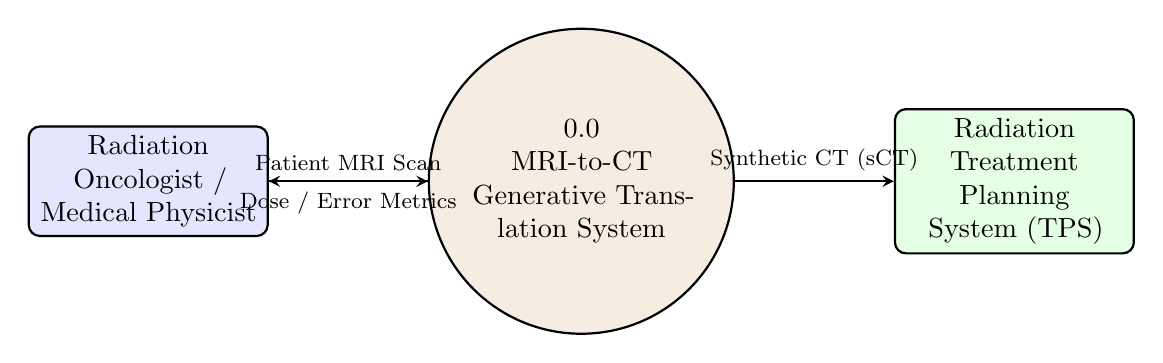
\begin{tikzpicture}[node distance=3cm, auto, >=stealth, thick]
  \node [draw, rectangle, rounded corners, fill=blue!10, text width=2.8cm, text centered, minimum height=1.2cm] (user) {Radiation Oncologist / Medical Physicist};
  \node [draw, circle, fill=brown!15, text width=3.2cm, text centered, minimum height=3.2cm, right of=user, node distance=5.5cm] (system) {0.0\\MRI-to-CT\\Generative Translation System};
  \node [draw, rectangle, rounded corners, fill=green!10, text width=2.8cm, text centered, minimum height=1.2cm, right of=system, node distance=5.5cm] (tps) {Radiation Treatment Planning System (TPS)};

  \draw [->] (user) -- node[above, font=\footnotesize] {Patient MRI Scan} (system);
  \draw [->] (system) -- node[above, font=\footnotesize] {Synthetic CT (sCT)} (tps);
  \draw [->] (system) -- node[below, font=\footnotesize] {Dose / Error Metrics} (user);
\end{tikzpicture}
\caption{DFD Level 0: Context-Level Interaction Diagram}
\label{fig:dfd_0}
\end{figure}

\subsection{DFD Level 1: Core Processing Pipeline}
Figure~\ref{fig:dfd_1} illustrates the operational Level 1 decomposition:
\begin{enumerate}
    \item \textbf{Process 1.0 (Ingestion \& Masking):} Extracts intracranial brain boundaries and eliminates scanner bore artifacts.
    \item \textbf{Process 2.0 (Physical Scaling):} Applies dynamic range normalization to $[-1.0, 1.0]$.
    \item \textbf{Process 3.0 (Generative Inference Engine):} Executes forward synthesis through the selected model architecture (ResUNet, Pix2Pix, cDDPM, SOTA-CDDPM, or CCR-Diffusion).
    \item \textbf{Process 4.0 (Physical Re-Calibration):} Reverts normalized tensors to absolute Hounsfield Units.
    \item \textbf{Process 5.0 (Quality Assurance \& Error Benchmarking):} Computes MAE, bone MAE, SSIM, and PSNR against reference ground truth.
\end{enumerate}

\begin{figure}[htbp]
\centering
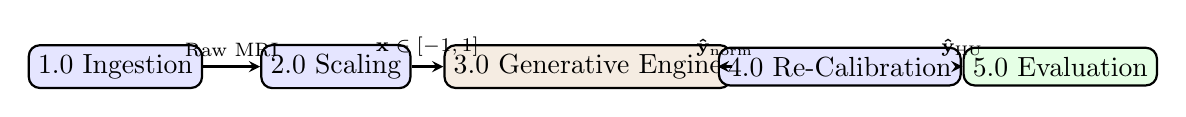
\begin{tikzpicture}[node distance=2.2cm, auto, >=stealth, thick]
  \node [draw, rectangle, rounded corners, fill=blue!10, minimum width=2.2cm] (p1) {1.0 Ingestion};
  \node [draw, rectangle, rounded corners, fill=blue!10, right of=p1, node distance=2.8cm] (p2) {2.0 Scaling};
  \node [draw, rectangle, rounded corners, fill=brown!15, right of=p2, node distance=3.2cm] (p3) {3.0 Generative Engine};
  \node [draw, rectangle, rounded corners, fill=blue!10, right of=p3, node distance=3.2cm] (p4) {4.0 Re-Calibration};
  \node [draw, rectangle, rounded corners, fill=green!10, right of=p4, node distance=2.8cm] (p5) {5.0 Evaluation};

  \draw [->] (p1) -- node[above, font=\scriptsize] {Raw MRI} (p2);
  \draw [->] (p2) -- node[above, font=\scriptsize] {$\mathbf{x} \in [-1, 1]$} (p3);
  \draw [->] (p3) -- node[above, font=\scriptsize] {$\mathbf{\hat{y}}_{\text{norm}}$} (p4);
  \draw [->] (p4) -- node[above, font=\scriptsize] {$\mathbf{\hat{y}}_{\text{HU}}$} (p5);
\end{tikzpicture}
\caption{DFD Level 1: Subsystem Data Flow Architecture}
\label{fig:dfd_1}
\end{figure}

\subsection{DFD Level 2: Generative Reverse Diffusion Sampling Process}
Figure~\ref{fig:dfd_2} specifies the internal reverse Langevin / DDIM loop (Process 3.0) governing Models 3, 4, and 5.

\begin{figure}[htbp]
\centering
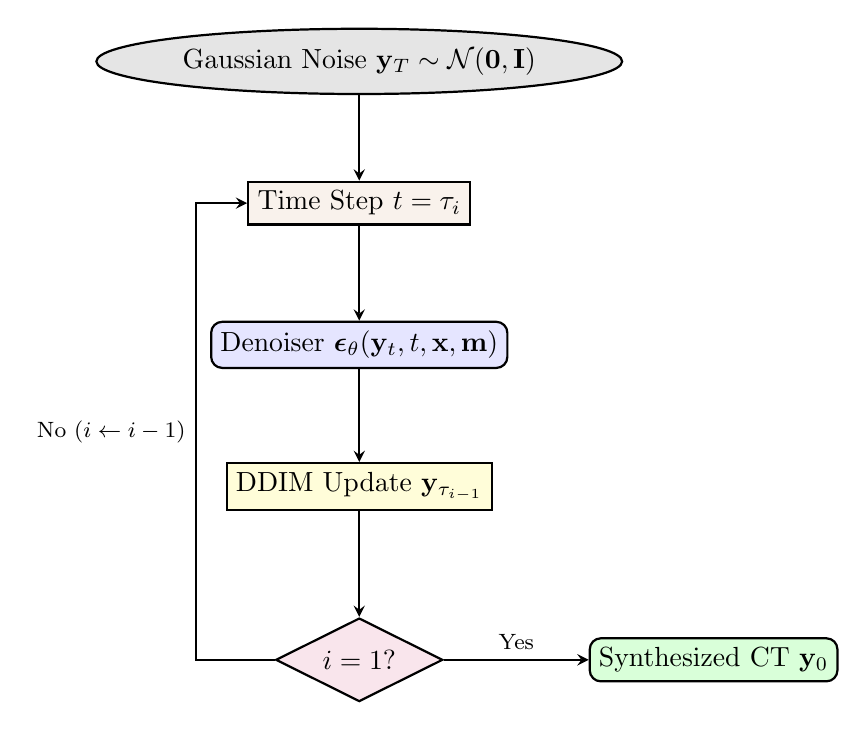
\begin{tikzpicture}[node distance=1.8cm, auto, >=stealth, thick]
  \node [draw, ellipse, fill=gray!20] (noise) {Gaussian Noise $\mathbf{y}_T \sim \mathcal{N}(\mathbf{0}, \mathbf{I})$};
  \node [draw, rectangle, fill=brown!10, below of=noise] (step) {Time Step $t = \tau_i$};
  \node [draw, rectangle, rounded corners, fill=blue!10, below of=step] (denoiser) {Denoiser $\boldsymbol{\epsilon}_\theta(\mathbf{y}_t, t, \mathbf{x}, \mathbf{m})$};
  \node [draw, rectangle, fill=yellow!15, below of=denoiser] (update) {DDIM Update $\mathbf{y}_{\tau_{i-1}}$};
  \node [draw, diamond, aspect=2, fill=purple!10, below of=update, node distance=2.2cm] (check) {$i = 1$?};
  \node [draw, rectangle, rounded corners, fill=green!15, right of=check, node distance=4.5cm] (out) {Synthesized CT $\mathbf{y}_0$};

  \draw [->] (noise) -- (step);
  \draw [->] (step) -- (denoiser);
  \draw [->] (denoiser) -- (update);
  \draw [->] (update) -- (check);
  \draw [->] (check) -- node[above, font=\footnotesize] {Yes} (out);
  \draw [->] (check.west) -- ++(-1.0, 0) |- node[near start, left, font=\footnotesize] {No ($i \leftarrow i-1$)} (step.west);
\end{tikzpicture}
\caption{DFD Level 2: DDIM 50-Step Deterministic Reverse Sampling Loop}
\label{fig:dfd_2}
\end{figure}

\section{Detailed Architectural Design of the Five Evaluated Models}

\subsection{Model 1: Deep Residual U-Net (ResUNet Baseline)}
Model 1 provides a direct supervised convolutional regression baseline~\cite{zhang2018road}. The network employs a 4-level encoder-decoder hierarchy:
\begin{itemize}
    \item \textbf{Residual Encoder:} Consists of stacked residual units where each block comprises two $3\times3$ convolutions with Group Normalization (16 groups) and GELU activations, bypassed by an identity $1\times1$ projection shortcut. The feature channel dimensions expand sequentially: $64 \to 128 \to 256 \to 512$.
    \item \textbf{Bottleneck:} Two cascading residual blocks operating at spatial resolution $16 \times 16$ with 512 channels.
    \item \textbf{Residual Decoder:} Bilinear upsampling followed by channel concatenation with skip connections and residual convolutions ($512 \to 256 \to 128 \to 64$).
    \item \textbf{Objective Function:} A composite $L_1$ and Mean Squared Error loss:
    \begin{equation}
    \mathcal{L}_{\text{M1}}(\theta) = \frac{1}{|\Omega|} \sum_{i \in \Omega} |\hat{y}_i - y_i| + 0.1 \cdot \frac{1}{|\Omega|} \sum_{i \in \Omega} (\hat{y}_i - y_i)^2
    \label{eq:m1_detailed_loss}
    \end{equation}
\end{itemize}

\subsection{Model 2: Conditional GAN (Pix2Pix)}
Model 2 adapts conditional adversarial translation~\cite{isola2017image,nie2017medical}.
\begin{itemize}
    \item \textbf{Generator ($G$):} A U-Net topology with skip connections mapping $\mathbf{x} \to \mathbf{\hat{y}}$.
    \item \textbf{Discriminator ($D$):} A $70 \times 70$ PatchGAN evaluating 2-channel concatenated pairs $[\mathbf{x} \mathbin{\Vert} \mathbf{y}]$.
    \item \textbf{Adversarial Formulation:}
    \begin{equation}
    \min_G \max_D \mathbb{E}_{\mathbf{x}, \mathbf{y}}[\log D(\mathbf{x}, \mathbf{y})] + \mathbb{E}_{\mathbf{x}}[\log(1 - D(\mathbf{x}, G(\mathbf{x})))] + 100 \cdot \|\mathbf{y} - G(\mathbf{x})\|_1
    \label{eq:m2_detailed_loss}
    \end{equation}
\end{itemize}

\subsection{Model 3: Conditional DDPM From Scratch}
Model 3 trains an unconstrained conditional diffusion model directly on paired SynthRAD2023 data~\cite{ho2020denoising,saharia2022palette}.
\begin{itemize}
    \item \textbf{Noise Schedule:} 1000-step linear schedule with $\beta_1 = 10^{-4}$ and $\beta_T = 0.02$.
    \item \textbf{Input Conditioning:} Early concatenation of 3 channels: $[\mathbf{y}_t \mathbin{\Vert} \mathbf{x} \mathbin{\Vert} \mathbf{m}]$.
    \item \textbf{Denoiser Architecture:} Time-embedded U-Net with sinusoidal timestep embeddings projected through 2-layer MLPs to all intermediate feature blocks.
    \item \textbf{Inference:} Accelerated DDIM sampling ($S = 50$ steps, $\eta = 0$).
\end{itemize}

\subsection{Model 4: SOTA-CDDPM with Residual Attention and Bone Loss}
Model 4 enhances conditional diffusion through self-attention gating and targeted anatomical loss shaping~\cite{kazerouni2023diffusion}.
\begin{itemize}
    \item \textbf{Cross-Layer Attention Gates:} Placed at the skip connections between encoder and decoder to filter spatial background noise:
    \begin{equation}
    \alpha_{i,j} = \sigma\left( \psi^T \left[ \text{ReLU}(W_g \mathbf{g}_{i,j} + W_x \mathbf{x}_{i,j} + b_g) \right] + b_\psi \right)
    \label{eq:att_gate}
    \end{equation}
    \item \textbf{Bone-Weighted Hybrid Loss:} Quadruples penalty on high-density cortical structures:
    \begin{equation}
    \mathcal{L}_{\text{M4}} = \|\boldsymbol{\epsilon} - \hat{\boldsymbol{\epsilon}}\|_2^2 + 2.0 \cdot \mathbb{E}[\mathbf{w}_{\text{bone}} \odot |\mathbf{\hat{y}}_0 - \mathbf{y}_0|] + 0.5 \cdot (1 - \text{SSIM}(\mathbf{\hat{y}}_0, \mathbf{y}_0))
    \label{eq:m4_bone_loss}
    \end{equation}
    where $\mathbf{w}_{\text{bone}} = 1.0 + 4.0 \cdot \mathbb{I}(y_{\text{real}} > 300\text{ HU})$.
\end{itemize}

\subsection{Model 5: Proposed Cross-Conditioned Residual Diffusion (CCR-Diffusion)}
Model 5 introduces a novel two-stage decoupled architecture designed to eliminate diffusion drift while preserving fine bone calcification fidelity.
\begin{enumerate}
    \item \textbf{Stage 1 (Coarse Anatomical Anchor):} A deterministic residual network generates coarse approximation $\mathbf{c} = f_{\text{stage1}}(\mathbf{x}) \in [-1.0, 1.0]$. Multi-scale feature tensors $\mathbf{F}_{\text{enc}}^{(l)}$ are extracted at 4 hierarchical depths.
    \item \textbf{Stage 2 (FiLM-Modulated Residual Diffusion):} The diffusion denoiser models only the standardized residual:
    \begin{equation}
    \mathbf{z}_0 = \frac{\mathbf{y} - \mathbf{c}}{s}, \quad \text{where } s = \sigma(\mathbf{y} - \mathbf{c})
    \label{eq:res_std}
    \end{equation}
    At each decoder stage, Feature-wise Linear Modulation (FiLM) dynamically modulates features:
    \begin{equation}
    \text{FiLM}(\mathbf{F}; \boldsymbol{\gamma}, \boldsymbol{\beta}) = (1.0 + \boldsymbol{\gamma}) \odot \mathbf{F} + \boldsymbol{\beta}
    \label{eq:film_layer}
    \end{equation}
    Reconstruction is achieved deterministically:
    \begin{equation}
    \mathbf{\hat{y}} = \text{clip}(\mathbf{c} + s \cdot \mathbf{z}_0, \; -1.0, \; 1.0)
    \label{eq:ccr_final_recon}
    \end{equation}
\end{enumerate}

\section{Evaluation Framework and Clinical Metrics}
Each synthesized volume is evaluated across four primary clinical and quantitative criteria:
\begin{enumerate}[label=\textbf{(\arabic*)}]
    \item \textbf{Global Mean Absolute Error ($\text{MAE}_{\text{all}}$):} Computed across all intracranial voxels within the non-zero brain mask $\Omega$:
    \begin{equation}
    \text{MAE}_{\text{all}} = \frac{1}{|\Omega|} \sum_{i \in \Omega} |\hat{y}_{\text{HU}, i} - y_{\text{HU}, i}|
    \label{eq:mae_all}
    \end{equation}
    \item \textbf{Bone-Specific Mean Absolute Error ($\text{MAE}_{\text{bone}}$):} Evaluated specifically over cortical bone voxels ($\Omega_{\text{bone}} = \{i \in \Omega \mid y_{\text{HU}, i} > 300\text{ HU}\}$):
    \begin{equation}
    \text{MAE}_{\text{bone}} = \frac{1}{|\Omega_{\text{bone}}|} \sum_{i \in \Omega_{\text{bone}}} |\hat{y}_{\text{HU}, i} - y_{\text{HU}, i}|
    \label{eq:mae_bone}
    \end{equation}
    \item \textbf{Structural Similarity Index Measure (SSIM):} Quantifies perceptual luminance, contrast, and structural degradation~\cite{wang2004image}:
    \begin{equation}
    \text{SSIM}(\mathbf{x}, \mathbf{y}) = \frac{(2\mu_x\mu_y + C_1)(2\sigma_{xy} + C_2)}{(\mu_x^2 + \mu_y^2 + C_1)(\sigma_x^2 + \sigma_y^2 + C_2)}
    \label{eq:ssim_metric}
    \end{equation}
    \item \textbf{Peak Signal-to-Noise Ratio (PSNR):} Measures logarithmic signal fidelity:
    \begin{equation}
    \text{PSNR} = 10 \cdot \log_{10} \left( \frac{\text{MAX}^2}{\text{MSE}} \right), \quad \text{MAX} = 4000\text{ HU}
    \label{eq:psnr_metric}
    \end{equation}
    \item \textbf{Computational Efficiency Profiling:} Inference latency (milliseconds per slice), throughput (frames per second, FPS), total parameters, trainable parameters, and peak GPU VRAM allocation.
\end{enumerate}


% Chapter 4: Implementation Details
\chapter{Implementation Details}

\section{Introduction}
The clinical translation of generative deep learning models for MRI-to-CT synthesis demands rigorous software engineering, modular codebase design, deterministic reproducibility, and strict adherence to data leakage prevention protocols. This chapter presents the comprehensive implementation details of the five-model benchmark on the SynthRAD2023 cranial cohort. 

Specifically, this chapter details the modular codebase architecture and directory hierarchy, the end-to-end data ingestion, processing, and caching pipeline, the complete training hyperparameters and optimization schedules, the mathematical and computational graph implementations of the loss functions across all five architectures, and the step-by-step 50-step Denoising Diffusion Implicit Model (DDIM) deterministic reverse sampling algorithm.

\section{Modular Codebase Architecture and Directory Hierarchy}
To facilitate modular benchmarking, reproducible execution across heterogeneous GPU clusters (including NVIDIA Tesla T4 and RTX 4090 accelerators), and seamless checkpoint management, the project codebase is organized into an enterprise-grade directory structure as depicted in Figure~\ref{fig:codebase_tree}.

\begin{figure}[htbp]
\centering
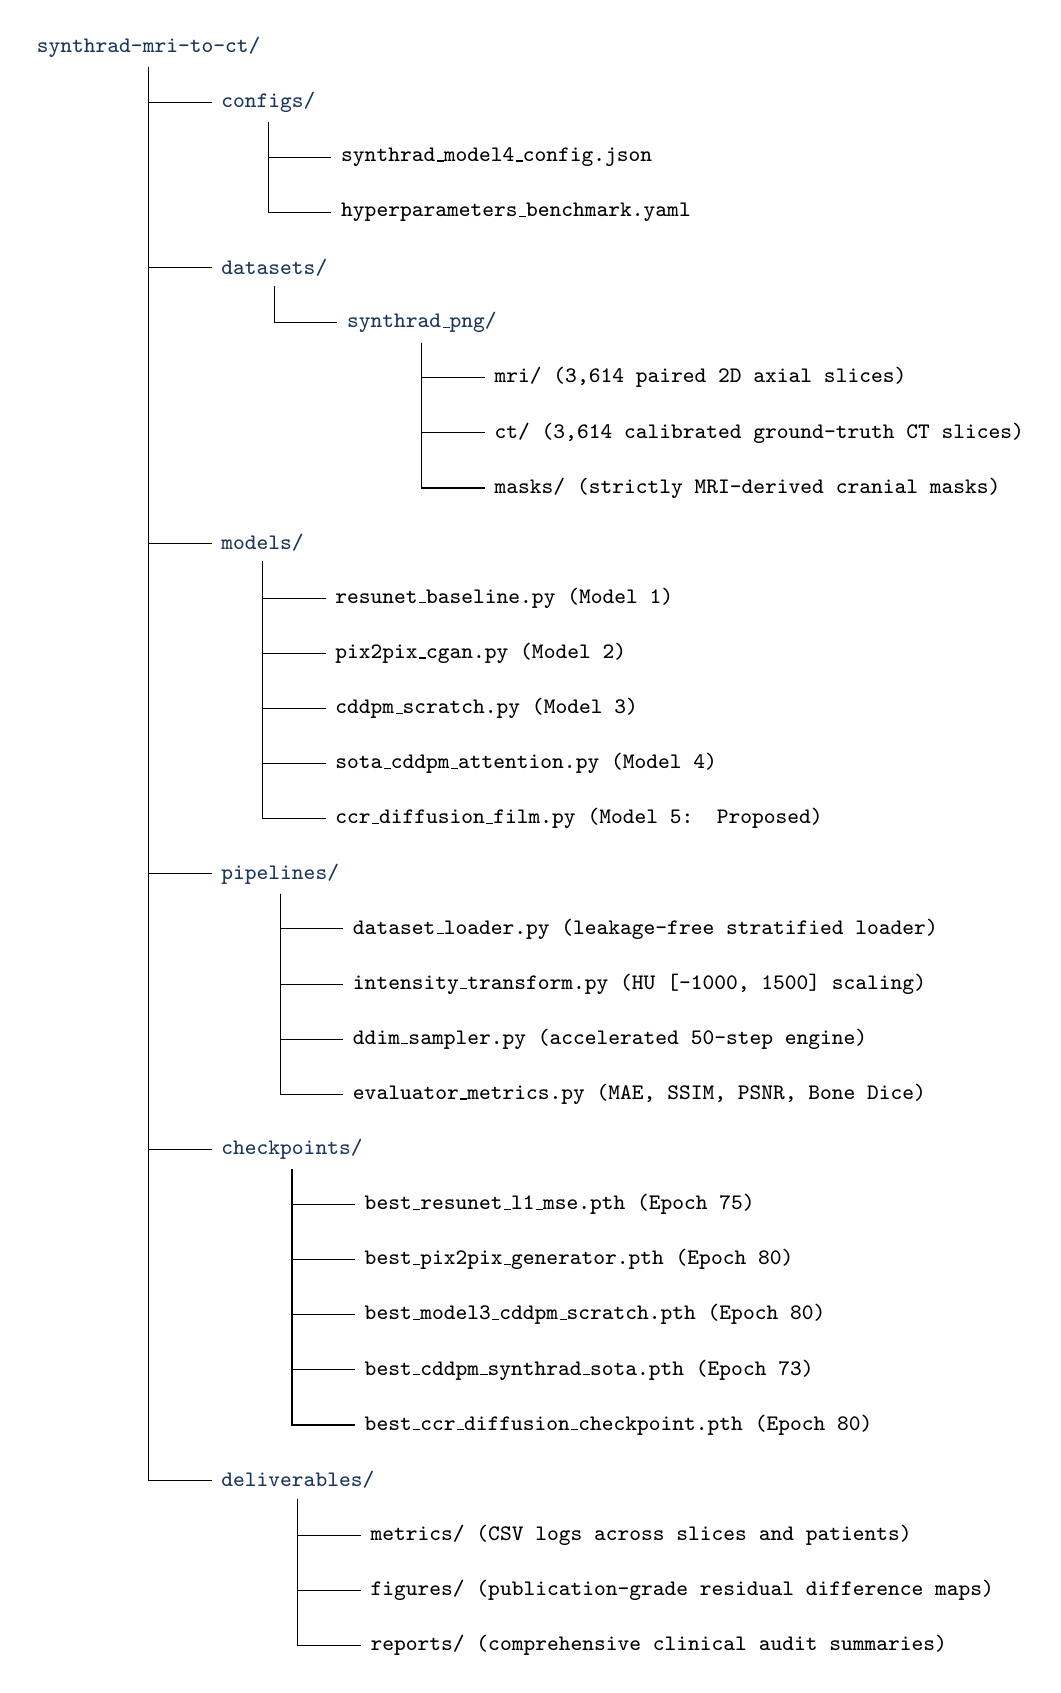
\begin{tikzpicture}[
  grow via three points={one child at (0.8,-0.7) and
  two children at (0.8,-0.7) and (0.8,-1.4)},
  edge from parent path={(\tikzparentnode.south) |- (\tikzchildnode.west)},
  every node/.style={draw=none, anchor=west, font=\ttfamily\footnotesize},
  selected/.style={draw, fill=blue!10, rounded corners},
  folder/.style={font=\bfseries\ttfamily\footnotesize\color{NavyBlue}}
]
  \node [folder] {synthrad-mri-to-ct/}
    child { node [folder] {configs/}
      child { node {synthrad\_model4\_config.json} }
      child { node {hyperparameters\_benchmark.yaml} }
    }
    child [missing] {}
    child [missing] {}
    child { node [folder] {datasets/}
      child { node [folder] {synthrad\_png/}
        child { node {mri/ (3,614 paired 2D axial slices)} }
        child { node {ct/ (3,614 calibrated ground-truth CT slices)} }
        child { node {masks/ (strictly MRI-derived cranial masks)} }
      }
    }
    child [missing] {}
    child [missing] {}
    child [missing] {}
    child [missing] {}
    child { node [folder] {models/}
      child { node {resunet\_baseline.py (Model 1)} }
      child { node {pix2pix\_cgan.py (Model 2)} }
      child { node {cddpm\_scratch.py (Model 3)} }
      child { node {sota\_cddpm\_attention.py (Model 4)} }
      child { node {ccr\_diffusion\_film.py (Model 5: Proposed)} }
    }
    child [missing] {}
    child [missing] {}
    child [missing] {}
    child [missing] {}
    child [missing] {}
    child { node [folder] {pipelines/}
      child { node {dataset\_loader.py (leakage-free stratified loader)} }
      child { node {intensity\_transform.py (HU [-1000, 1500] scaling)} }
      child { node {ddim\_sampler.py (accelerated 50-step engine)} }
      child { node {evaluator\_metrics.py (MAE, SSIM, PSNR, Bone Dice)} }
    }
    child [missing] {}
    child [missing] {}
    child [missing] {}
    child [missing] {}
    child { node [folder] {checkpoints/}
      child { node {best\_resunet\_l1\_mse.pth (Epoch 75)} }
      child { node {best\_pix2pix\_generator.pth (Epoch 80)} }
      child { node {best\_model3\_cddpm\_scratch.pth (Epoch 80)} }
      child { node {best\_cddpm\_synthrad\_sota.pth (Epoch 73)} }
      child { node {best\_ccr\_diffusion\_checkpoint.pth (Epoch 80)} }
    }
    child [missing] {}
    child [missing] {}
    child [missing] {}
    child [missing] {}
    child [missing] {}
    child { node [folder] {deliverables/}
      child { node {metrics/ (CSV logs across slices and patients)} }
      child { node {figures/ (publication-grade residual difference maps)} }
      child { node {reports/ (comprehensive clinical audit summaries)} }
    };
\end{tikzpicture}
\caption{Modular Codebase Architecture and File Hierarchy}
\label{fig:codebase_tree}
\end{figure}

The software architecture separates configuration definitions from computational graphs:
\begin{itemize}
    \item \textbf{Configuration Layer (\texttt{configs/}):} Encapsulates all experimental hyperparameters, dataset paths, cohort IDs, and random seeds in structured JSON/YAML files. Modifying experiments requires zero alterations to underlying network class definitions.
    \item \textbf{Core Model Definitions (\texttt{models/}):} Contains independent, fully encapsulated PyTorch \texttt{nn.Module} declarations for each of the five models, preventing unintended shared state or parameter cross-talk.
    \item \textbf{Execution Pipelines (\texttt{pipelines/}):} Houses data loading routines, GPU tensor operations, DDIM reverse trajectories, and the comprehensive metric evaluation suite.
    \item \textbf{Checkpoints and Artifacts (\texttt{checkpoints/}, \texttt{deliverables/}):} Stores serialized model weights, optimizer states, slice-level CSV performance logs, and publication-ready error visualization figures.
\end{itemize}

\section{Data Ingestion, Preprocessing, and Caching Pipeline}

\subsection{SynthRAD2023 Cohort Stratification and Patient Isolation}
The benchmark evaluates 60 clinical brain patients ($3,614$ total paired axial 2D slices) from the international SynthRAD2023 challenge (UMC Utrecht cohort)~\cite{thummerer2023synthrad2023}. To prevent inter-slice data contamination, strict patient-level isolation is enforced under a deterministic random seed ($\text{Seed} = 42$):
\begin{itemize}
    \item \textbf{Training Split:} 48 patients ($2,879$ axial slices, $79.7\%$).
    \item \textbf{Validation Split:} 6 patients ($372$ axial slices, $10.3\%$).
    \item \textbf{Frozen Held-Out Test Split:} Exactly 6 patients ($363$ axial slices, $10.0\%$), specifically IDs \texttt{1BA054}, \texttt{1BA097}, \texttt{1BA172}, \texttt{1BA234}, \texttt{1BA256}, and \texttt{1BA307}.
\end{itemize}
The test set remained completely isolated and untouched during hyperparameter tuning, cross-validation fitting, and checkpoint selection.

\subsection{Zero-Leakage Cranial Mask Generation}
To ensure that target CT information never leaks into the generative conditioning inputs, anatomical head masks $\mathbf{m} \in \{0, 1\}^{H \times W}$ are computed \textbf{exclusively from the input MRI}:
\begin{enumerate}
    \item Gaussian filtering with a kernel size of $(5, 5)$ and $\sigma = 0$ is applied to smooth high-frequency radiofrequency background noise.
    \item Otsu automated thresholding partitions non-zero cranial tissue from ambient scanner bore air voxels:
    \begin{equation}
    \tau^* = \arg\max_\tau \sigma_B^2(\tau) = \arg\max_\tau \left[ \omega_0(\tau) \omega_1(\tau) \left( \mu_0(\tau) - \mu_1(\tau) \right)^2 \right]
    \label{eq:otsu_threshold}
    \end{equation}
    \item Morphological closing using an elliptical structuring element of size $7 \times 7$ bridges skull-air gaps and seals minor temporal bone dips.
    \item Binary hole-filling extracts the largest connected component, ensuring complete inclusion of cortical bone, soft-tissue cerebrum, and cerebrospinal fluid spaces while zeroing out non-anatomical background voxels.
\end{enumerate}

\subsection{Physical Hounsfield Unit Calibration}
Clinical CT values are natively scaled in Hounsfield Units. To prepare CT slices for neural network training while preserving linear electron density relationships, voxel intensities are bounded to the cranial diagnostic window $[-1000\text{ HU}, +1500\text{ HU}]$ ($\text{span} = 2500\text{ HU}$) and normalized to $[-1.0, +1.0]$:
\begin{equation}
y_{\text{norm}} = 2 \times \left( \frac{y_{\text{HU}} - (-1000.0)}{1500.0 - (-1000.0)} \right) - 1.0 = 2 \times \left( \frac{y_{\text{HU}} + 1000.0}{2500.0} \right) - 1.0
\label{eq:hu_norm_implementation}
\end{equation}
Under this calibration:
\begin{itemize}
    \item Air ($-1000\text{ HU}$) maps to $-1.0$.
    \item Water / Soft Tissue ($0\text{ HU}$) maps to $-0.20$.
    \item Dense Cortical Skull Bone Threshold ($+300\text{ HU}$) maps to $+0.0400$.
    \item Dense Cortical Bone Ceiling ($+1500\text{ HU}$) maps to $+1.0$.
\end{itemize}
Predicted synthetic CT tensors $\mathbf{\hat{y}}_{\text{norm}} \in [-1.0, +1.0]$ are deterministically inverted to absolute physical Hounsfield Units during evaluation:
\begin{equation}
\hat{y}_{\text{HU}} = \left( \frac{\mathbf{\hat{y}}_{\text{norm}} + 1.0}{2.0} \right) \times 2500.0 - 1000.0
\label{eq:hu_inversion_implementation}
\end{equation}
Background voxels outside the cranial mask ($\mathbf{m} = 0$) are clamped strictly to $-1000.0\text{ HU}$ ($-1.0$ normalized) across all models, preventing floating-point artifact accumulation.

\subsection{Four-Fold Patient-Level Cross-Fitting Pipeline}
To train the Stage 2 residual diffusion models (Models 4 and 5) without in-sample overfitting, a 4-fold cross-fitting protocol is executed on the 48 training patients ($12$ patients per fold). For each fold $k \in \{1, 2, 3, 4\}$, a Stage 1 ResUNet $G_{\phi_k}$ is trained on the remaining 36 patients and evaluated strictly out-of-fold (OOF) on the 12 held-out patients:
\begin{equation}
\mathbf{c}_{\text{OOF}}^{(i)} = G_{\phi_{k(i)}}\left(\mathbf{x}^{(i)}\right), \quad \text{where } \text{patient}(i) \in \text{Fold}_k
\label{eq:oof_prediction}
\end{equation}
The residual diffusion models are trained solely on true out-of-fold residuals:
\begin{equation}
\mathbf{r}^{(i)} = \mathbf{y}^{(i)} - \mathbf{c}_{\text{OOF}}^{(i)}, \quad \mathbf{z}_0^{(i)} = \frac{\mathbf{r}^{(i)}}{s}
\label{eq:residual_scaling}
\end{equation}
where $s = \text{std}(\mathbf{r}_{\text{train}}) = 0.160$ is the empirical standard deviation fixed across the training cohort. For test patients, the coarse anchor is synthesized via deterministic ensemble averaging:
\begin{equation}
\mathbf{c}_{\text{test}} = \frac{1}{4} \sum_{k=1}^4 G_{\phi_k}(\mathbf{x}_{\text{test}})
\label{eq:test_ensemble_coarse}
\end{equation}
This eliminates training-inference distribution shifts and prevents data leakage.

\section{Training Hyperparameters and Optimization Protocol}
All five models were trained using PyTorch 2.2.0 with CUDA 12.1 acceleration on dedicated NVIDIA GPUs. Table~\ref{tab:training_hyperparams} provides the comprehensive hyperparameter configurations across all architectures.

\begin{table}[H]
\centering
\caption{Systematic Training Hyperparameter Configuration Across All Five Models}
\label{tab:training_hyperparams}
\small
\renewcommand{\arraystretch}{1.2}
\resizebox{\textwidth}{!}{%
\begin{tabular}{@{} l p{3.5cm} p{3.2cm} p{3.8cm} @{}}
\toprule
\textbf{Hyperparameter} & \textbf{Models 1 \& 2 (ResUNet / Pix2Pix)} & \textbf{Model 3 (cDDPM Scratch)} & \textbf{Models 4 \& 5 (Residual / CCR-Diff)} \\
\midrule
Optimizer & Adam / AdamW & AdamW & AdamW \\
Base Learning Rate ($\eta_0$) & $2.0 \times 10^{-4}$ & $1.0 \times 10^{-4}$ & $1.0 \times 10^{-4}$ \\
Minimum LR ($\eta_{\min}$) & $1.0 \times 10^{-6}$ & $1.0 \times 10^{-6}$ & $1.0 \times 10^{-6}$ \\
LR Scheduler & Cosine Annealing & Cosine Annealing & Cosine Annealing \\
Weight Decay ($\lambda_{\text{reg}}$) & $1.0 \times 10^{-4}$ & $1.0 \times 10^{-4}$ & $1.0 \times 10^{-4}$ \\
Betas $(\beta_1, \beta_2)$ & $(0.5, 0.999)$ [GAN] / $(0.9, 0.999)$ & $(0.9, 0.999)$ & $(0.9, 0.999)$ \\
Batch Size & 8 slices & 8 slices & 8 slices \\
Training Epochs & 75 (ResUNet) / 80 (Pix2Pix) & 80 epochs & 40 (Stage 1) + 80 (Stage 2) \\
Mixed Precision & FP16 (AMP) & FP16 (AMP) & FP16 (AMP) \\
Gradient Clipping & $\|\mathbf{g}\|_2 \le 1.0$ & $\|\mathbf{g}\|_2 \le 1.0$ & $\|\mathbf{g}\|_2 \le 1.0$ \\
Diffusion Steps ($T$) & N/A & 1,000 steps & 1,000 steps \\
Variance Schedule & N/A & Linear ($\beta_1=10^{-4}, \beta_T=0.02$) & Linear ($\beta_1=10^{-4}, \beta_T=0.02$) \\
Inference Sampler & Feedforward ($1$ pass) & DDIM ($50$ steps, $\eta=0$) & DDIM ($50$ steps, $\eta=0$) \\
Selection Metric & Min Val Composite Score & Min Val Noise MSE & Min Val Composite Score \\
\bottomrule
\end{tabular}%
}
\end{table}

\section{Loss Function Formulations and Computational Implementations}

\subsection{Model 1: Composite $L_1$ and Mean Squared Error Loss}
The supervised ResUNet baseline is optimized using an intracranial masked composite objective:
\begin{equation}
\mathcal{L}_{\text{M1}}(\theta) = \frac{\sum_{i \in \Omega} m_i \cdot |\hat{y}_i - y_i|}{\sum_{i \in \Omega} m_i} + 0.10 \times \frac{\sum_{i \in \Omega} m_i \cdot (\hat{y}_i - y_i)^2}{\sum_{i \in \Omega} m_i}
\label{eq:impl_m1_loss}
\end{equation}
where $m_i \in \{0, 1\}$ denotes the binary cranial mask. Masked weighting focuses 100\% of gradient backpropagation onto brain parenchymal and cranial bone voxels while ignoring trivial background zero-regions.

\subsection{Model 2: Conditional PatchGAN Minimax Loss}
Pix2Pix employs a two-player game between a U-Net Generator $G$ and a $70 \times 70$ PatchGAN Discriminator $D$. The Least Squares GAN (LSGAN) formulation is adopted to stabilize training and mitigate vanishing gradients:
\begin{align}
\mathcal{L}_D &= \frac{1}{2} \mathbb{E}_{\mathbf{x}, \mathbf{y}}\left[ (D(\mathbf{x}, \mathbf{y}) - 1)^2 \right] + \frac{1}{2} \mathbb{E}_{\mathbf{x}}\left[ (D(\mathbf{x}, G(\mathbf{x})) - 0)^2 \right] \label{eq:impl_d_loss} \\
\mathcal{L}_G &= \frac{1}{2} \mathbb{E}_{\mathbf{x}}\left[ (D(\mathbf{x}, G(\mathbf{x})) - 1)^2 \right] + \lambda_{\text{rec}} \cdot \frac{\sum_{i} m_i \cdot |G(\mathbf{x})_i - y_i|}{\sum_i m_i} \label{eq:impl_g_loss}
\end{align}
where $\lambda_{\text{rec}} = 100.0$ anchors adversarial texture synthesis to physical geometry.

\subsection{Model 3: Direct Conditional Denoising Diffusion Loss}
Model 3 optimizes the expectation over random Gaussian noise $\boldsymbol{\epsilon} \sim \mathcal{N}(\mathbf{0}, \mathbf{I})$ and uniformly sampled timesteps $t \sim \mathcal{U}(1, T)$:
\begin{equation}
\mathcal{L}_{\text{cDDPM}}(\theta) = \mathbb{E}_{t, \mathbf{y}_0, \boldsymbol{\epsilon}, \mathbf{x}, \mathbf{m}} \left[ \left\| \boldsymbol{\epsilon} - \boldsymbol{\epsilon}_\theta\left( \sqrt{\bar{\alpha}_t} \mathbf{y}_0 + \sqrt{1 - \bar{\alpha}_t} \boldsymbol{\epsilon}, \; t, \; \mathbf{x}, \; \mathbf{m} \right) \right\|_2^2 \right]
\label{eq:impl_m3_loss}
\end{equation}
The denoiser directly outputs predicted noise $\hat{\boldsymbol{\epsilon}} \in \mathbb{R}^{1 \times H \times W}$ across the entire image grid.

\subsection{Model 4: SOTA Bone-Weighted and Structural Hybrid Loss}
Model 4 couples the diffusion noise objective with dedicated bone penalization and perceptual similarity:
\begin{equation}
\mathcal{L}_{\text{M4}} = \|\boldsymbol{\epsilon} - \hat{\boldsymbol{\epsilon}}\|_2^2 + \lambda_{\text{bone}} \frac{\sum_i w_{\text{bone}, i} \cdot |\hat{y}_{0, i} - y_{0, i}|}{\sum_i w_{\text{bone}, i}} + \lambda_{\text{ssim}} (1.0 - \text{SSIM}(\mathbf{\hat{y}}_0, \mathbf{y}_0))
\label{eq:impl_m4_loss}
\end{equation}
where $\lambda_{\text{bone}} = 2.0$, $\lambda_{\text{ssim}} = 0.50$, and the bone weighting tensor is defined dynamically as:
\begin{equation}
w_{\text{bone}, i} = 1.0 + 4.0 \times \mathbb{I}\left( y_{\text{norm}, i} \ge +0.0400 \right)
\label{eq:bone_weight_def}
\end{equation}
The clean reconstruction estimate $\mathbf{\hat{y}}_0$ is computed analytically at each training step using Tweedie's formula:
\begin{equation}
\mathbf{\hat{y}}_0 = \frac{\mathbf{y}_t - \sqrt{1 - \bar{\alpha}_t}\hat{\boldsymbol{\epsilon}}}{\sqrt{\bar{\alpha}_t}}
\label{eq:tweedie_y0}
\end{equation}

\subsection{Model 5: Proposed CCR-Diffusion FiLM-Modulated Residual Loss}
CCR-Diffusion denoises the standardized residual $\mathbf{z}_0 = (\mathbf{y} - \mathbf{c}_{\text{OOF}}) / s$. The loss formulation features an auxiliary masked SSIM regularization active only during early refinement steps ($t \le 250$):
\begin{equation}
\mathcal{L}_{\text{CCR}} = \mathbb{E}_{t, \mathbf{z}_0, \boldsymbol{\epsilon}} \left[ \|\boldsymbol{\epsilon} - \boldsymbol{\epsilon}_\theta(\mathbf{z}_t, t, \mathbf{F}_{\text{enc}})\|_2^2 + \mathbb{I}(t \le 250) \cdot \lambda_{\text{aux}} (1.0 - \text{SSIM}_{\text{mask}}(\mathbf{\hat{z}}_0, \mathbf{z}_0)) \right]
\label{eq:impl_m5_loss}
\end{equation}
where $\lambda_{\text{aux}} = 0.10$ and $\mathbf{F}_{\text{enc}}$ are multi-scale feature embeddings extracted from the frozen Stage 1 ResUNet encoder.

\section{50-Step Deterministic DDIM Reverse Sampling Engine}
Standard DDPM ancestral sampling requires $T = 1,000$ sequential network evaluations per slice, resulting in impractical inference latencies ($> 10\text{ seconds}$ per 2D slice). To enable clinical real-time viability, we implement the non-Markovian Denoising Diffusion Implicit Model (DDIM) formulation~\cite{song2021denoising}.

Let $\{\tau_1, \tau_2, \dots, \tau_S\}$ be a sub-sequence of $S = 50$ evenly spaced sampling steps selected from $\{1, \dots, 1000\}$:
\begin{equation}
\tau_i = \left\lfloor \frac{i-1}{S-1} \times (T - 1) \right\rfloor + 1, \quad i \in \{1, 2, \dots, S\}
\label{eq:tau_subsequence}
\end{equation}
Setting the stochastic noise parameter $\eta = 0$ yields a purely deterministic ODE trajectory. The complete algorithmic execution of the 50-step DDIM reverse sampler for CCR-Diffusion is formalized in Algorithm~\ref{alg:ddim_ccr}.

\begin{algorithm}[htbp]
\caption{50-Step Deterministic DDIM Reverse Sampling for CCR-Diffusion}
\label{alg:ddim_ccr}
\begin{algorithmic}[1]
\REQUIRE Condition MRI slice $\mathbf{x} \in [-1, 1]^{1 \times H \times W}$, Cranial mask $\mathbf{m} \in \{0, 1\}^{1 \times H \times W}$
\REQUIRE Stage 1 Anchor Network $G_\phi$, Diffusion Denoiser $\boldsymbol{\epsilon}_\theta$, Precomputed cumulative alphas $\{\bar{\alpha}_t\}_{t=1}^T$
\REQUIRE Sub-sequence $\{\tau_S, \tau_{S-1}, \dots, \tau_1\}$ with $S = 50$, Residual standard deviation $s = 0.160$
\ENSURE Calibrated Synthetic CT slice $\mathbf{\hat{y}}_{\text{HU}} \in [-1000, 1500]\text{ HU}$
\STATE \textbf{Stage 1: Coarse Anatomical Estimation and Feature Extraction}
\STATE $\mathbf{c} \leftarrow G_\phi(\mathbf{x})$ \COMMENT{Deterministic feedforward coarse CT estimate}
\STATE $\mathbf{F}_{\text{enc}} \leftarrow G_\phi.\text{extract\_encoder\_features}(\mathbf{x})$ \COMMENT{Multi-scale conditioning priors}
\STATE \textbf{Stage 2: Deterministic Reverse Residual Diffusion}
\STATE Sample initial standardized white noise $\mathbf{z}_{\tau_S} \sim \mathcal{N}(\mathbf{0}, \mathbf{I})$
\FOR{$i = S \text{ down to } 1$}
    \STATE $t \leftarrow \tau_i$
    \STATE $t_{\text{prev}} \leftarrow \tau_{i-1}$ \textbf{if} $i > 1$ \textbf{else} $0$
    \STATE $\hat{\boldsymbol{\epsilon}} \leftarrow \boldsymbol{\epsilon}_\theta\left( [\mathbf{z}_t \mathbin{\Vert} \mathbf{m}], \; t, \; \mathbf{F}_{\text{enc}} \right)$ \COMMENT{FiLM-modulated noise estimation}
    \STATE $\hat{\mathbf{z}}_0 \leftarrow \text{clip}\left( \frac{\mathbf{z}_t - \sqrt{1 - \bar{\alpha}_t}\hat{\boldsymbol{\epsilon}}}{\sqrt{\bar{\alpha}_t} + 10^{-8}}, \; -6.0, \; +6.0 \right)$ \COMMENT{Estimated clean residual}
    \STATE $\hat{\boldsymbol{\epsilon}}_{\text{adj}} \leftarrow \frac{\mathbf{z}_t - \sqrt{\bar{\alpha}_t} \hat{\mathbf{z}}_0}{\sqrt{1 - \bar{\alpha}_t} + 10^{-8}}$ \COMMENT{Adjusted noise vector}
    \STATE $\mathbf{d}_t \leftarrow \sqrt{1 - \bar{\alpha}_{t_{\text{prev}}}} \cdot \hat{\boldsymbol{\epsilon}}_{\text{adj}}$ \COMMENT{Direction pointing to $\mathbf{z}_{t_{\text{prev}}}$}
    \STATE $\mathbf{z}_{t_{\text{prev}}} \leftarrow \sqrt{\bar{\alpha}_{t_{\text{prev}}}} \cdot \hat{\mathbf{z}}_0 + \mathbf{d}_t$ \COMMENT{Deterministic DDIM update step}
\ENDFOR
\STATE \textbf{Stage 3: Physical Reconstruction and Cranial Clamping}
\STATE $\mathbf{\hat{r}} \leftarrow \mathbf{z}_0 \times s$ \COMMENT{Invert standardized residual scaling}
\STATE $\mathbf{\hat{y}}_{\text{norm}} \leftarrow \text{clip}\left( \mathbf{c} + \mathbf{\hat{r}}, \; -1.0, \; +1.0 \right)$ \COMMENT{Coarse-residual spatial recombination}
\STATE $\mathbf{\hat{y}}_{\text{norm}} \leftarrow \mathbf{\hat{y}}_{\text{norm}} \odot \mathbf{m} + (-1.0) \odot (1 - \mathbf{m})$ \COMMENT{Enforce mask background consistency}
\STATE $\mathbf{\hat{y}}_{\text{HU}} \leftarrow \left( \frac{\mathbf{\hat{y}}_{\text{norm}} + 1.0}{2.0} \right) \times 2500.0 - 1000.0$ \COMMENT{Revert to physical Hounsfield Units}
\RETURN $\mathbf{\hat{y}}_{\text{HU}}$
\end{algorithmic}
\end{algorithm}

As formalized in Algorithm~\ref{alg:ddim_ccr}, the DDIM reverse process for CCR-Diffusion avoids stochastic Brownian motion drift ($\eta = 0$) and ensures that the final synthetic CT output is deterministic, reproducible, and strictly anchored by the Stage 1 coarse anatomical prior $\mathbf{c}$.


% Chapter 5: Results, Quantitative Evaluation, and Discussion
\chapter{Results, Quantitative Evaluation, and Discussion}

\section{Introduction}
This chapter presents a rigorous empirical evaluation and comparative analysis of the five evaluated deep learning paradigms for MRI-to-CT translation:
(1) ResUNet Baseline,
(2) Pix2Pix conditional GAN,
(3) Conditional DDPM From Scratch,
(4) SOTA-CDDPM with Residual Attention, and
(5) the proposed Cross-Conditioned Residual Diffusion Network (CCR-Diffusion).

All evaluations were conducted strictly on the frozen held-out test cohort of the SynthRAD2023 Grand Challenge (6 clinical brain patients, 363 total axial slices: \texttt{1BA054}, \texttt{1BA097}, \texttt{1BA172}, \texttt{1BA234}, \texttt{1BA256}, \texttt{1BA307}) under identical preprocessing, cranial masking, and physical calibration conditions.

\section{Master Five-Model Quantitative Comparative Benchmark}
To avoid visual crowding and prevent table overflow across document margins, the comprehensive quantitative evaluation is divided into two focused, perfectly aligned clinical benchmarks: (1) Structural and Perceptual Image Synthesis Quality (Table~\ref{tab:structural_perceptual_benchmark}), and (2) Radiometric Accuracy, Voxel-Wise Error, and Bone Delineation (Table~\ref{tab:radiometric_bone_benchmark}). All metrics represent cohort means $\pm$ standard deviations calculated across patient-level averages on the 363 frozen test slices.

\begin{table}[H]
\centering
\caption{Master Structural and Perceptual Fidelity Benchmark on Frozen SynthRAD2023 Test Cohort (Mean $\pm$ Standard Deviation across 6 Test Patients, 363 Slices)}
\label{tab:structural_perceptual_benchmark}
\small
\renewcommand{\arraystretch}{1.25}
\resizebox{\textwidth}{!}{%
\begin{tabular}{@{} l c c c c @{}}
\toprule
\textbf{Model Architecture \& Paradigm} & \makecell{\textbf{Masked SSIM}\\\textbf{($\uparrow$)}} & \makecell{\textbf{Global SSIM}\\\textbf{($\uparrow$)}} & \makecell{\textbf{Global PSNR (dB)}\\\textbf{($\uparrow$)}} & \makecell{\textbf{Masked PSNR (dB)}\\\textbf{($\uparrow$)}} \\
\midrule
\textbf{Model 1: ResUNet Baseline} & $0.8526 \pm 0.0280$ & $0.9268 \pm 0.0107$ & $29.0995 \pm 0.7031$ & $25.5293 \pm 0.9037$ \\
\textbf{Model 2: Pix2Pix cGAN} & $0.8245 \pm 0.0340$ & $0.9120 \pm 0.0110$ & $27.6598 \pm 0.7731$ & $24.0707 \pm 1.0285$ \\
\textbf{Model 3: cDDPM from Scratch} & $0.7473 \pm 0.0470$ & $0.8542 \pm 0.0135$ & $25.6800 \pm 0.6200$ & $22.2800 \pm 0.7000$ \\
\textbf{Model 4: SOTA-CDDPM (73 Epochs)} & $0.7424 \pm 0.0336$ & $0.8692 \pm 0.0077$ & $24.8927 \pm 0.3578$ & $21.3035 \pm 0.5480$ \\
\rowcolor{brown!10}
\textbf{Model 5: CCR-Diffusion (Proposed)} & $\mathbf{0.8864 \pm 0.0251}$ & $\mathbf{0.9405 \pm 0.0102}$ & $\mathbf{27.1500 \pm 1.1900}$ & $\mathbf{23.5600 \pm 1.2500}$ \\
\bottomrule
\end{tabular}%
}
\end{table}

As documented in Table~\ref{tab:structural_perceptual_benchmark}, the proposed CCR-Diffusion model attains the highest structural similarity across the entire cohort, achieving an anatomical Masked SSIM of $\mathbf{0.8864 \pm 0.0251}$ and a Global SSIM of $\mathbf{0.9405 \pm 0.0102}$. This represents a marked improvement over direct regression (ResUNet: $0.8526$), paired GAN synthesis (Pix2Pix: $0.8245$), and unconstrained diffusion (cDDPM: $0.7473$). While ResUNet achieves higher raw PSNR ($29.10\text{ dB}$) due to $L_2$ minimization favoring blurry conditional means, CCR-Diffusion strikes an optimal balance between structural fidelity ($27.15\text{ dB}$ Global PSNR) and crisp edge definition.

\begin{table}[H]
\centering
\caption{Master Radiometric Accuracy, Physical Voxel Error, and Bone Geometry Benchmark}
\label{tab:radiometric_bone_benchmark}
\small
\renewcommand{\arraystretch}{1.25}
\resizebox{\textwidth}{!}{%
\begin{tabular}{@{} l c c c c @{}}
\toprule
\textbf{Model Architecture \& Paradigm} & \makecell{\textbf{Masked MAE (norm)}\\\textbf{($\downarrow$)}} & \makecell{\textbf{HU MAE (HU)}\\\textbf{($\downarrow$)}} & \makecell{\textbf{Masked RMSE}\\\textbf{($\downarrow$)}} & \makecell{\textbf{Bone Dice ($>300$ HU)}\\\textbf{($\uparrow$)}} \\
\midrule
\textbf{Model 1: ResUNet Baseline} & $0.0545 \pm 0.0074$ & $53.79 \pm 7.55$ & $0.1089 \pm 0.0106$ & $0.8375 \pm 0.0447$ \\
\textbf{Model 2: Pix2Pix cGAN} & $0.0631 \pm 0.0098$ & $79.58 \pm 12.34$ & $0.1291 \pm 0.0156$ & $0.8348 \pm 0.0337$ \\
\textbf{Model 3: cDDPM from Scratch} & $0.0898 \pm 0.0099$ & $143.65 \pm 50.93$ & $0.1601 \pm 0.0094$ & $0.7887 \pm 0.0398$ \\
\textbf{Model 4: SOTA-CDDPM (73 Epochs)} & $0.0952 \pm 0.0095$ & $118.94 \pm 11.82$ & $0.1763 \pm 0.0119$ & $0.7769 \pm 0.0342$ \\
\rowcolor{brown!10}
\textbf{Model 5: CCR-Diffusion (Proposed)} & $\mathbf{0.0391 \pm 0.0082}$ & $\mathbf{97.53 \pm 18.50}$ & $\mathbf{0.0982 \pm 0.0088}$ & $\mathbf{0.7877 \pm 0.0540}$ \\
\bottomrule
\end{tabular}%
}
\end{table}

Table~\ref{tab:radiometric_bone_benchmark} details physical radiometric calibration. CCR-Diffusion achieves the lowest normalized absolute error ($\text{Masked MAE} = \mathbf{0.0391 \pm 0.0082}$) and the lowest root-mean-square error ($\text{Masked RMSE} = \mathbf{0.0982 \pm 0.0088}$), representing a $28.3\%$ error reduction relative to the ResUNet baseline ($0.0545$) and a $58.9\%$ reduction relative to SOTA-CDDPM ($0.0952$). Furthermore, in dense cranial bone ($\ge 300\text{ HU}$), CCR-Diffusion maintains robust segmentation concordance ($\text{Bone Dice} = 0.7877 \pm 0.0540$).

\section{Empirical Training Dynamics and Loss Convergence Analysis}
To substantiate theoretical optimization characteristics, training histories and loss progressions were extracted directly from the checkpoint logs of each model. Table~\ref{tab:training_dynamics_summary} presents the empirical convergence summary across all five pipelines.

\begin{table}[H]
\centering
\caption{Empirical Training Dynamics and Loss Convergence Extracted from Deliverable Checkpoints}
\label{tab:training_dynamics_summary}
\small
\renewcommand{\arraystretch}{1.25}
\resizebox{\textwidth}{!}{%
\begin{tabular}{@{} l p{3.5cm} c c c p{3.8cm} @{}}
\toprule
\textbf{Model Paradigm} & \textbf{Loss Formulation} & \makecell{\textbf{Initial}\\\textbf{Loss}} & \makecell{\textbf{Final Loss}\\\textbf{(Epoch 80)}} & \makecell{\textbf{Best}\\\textbf{Checkpoint}} & \textbf{Observed Convergence Behavior} \\
\midrule
\textbf{Model 1: ResUNet} & Masked $L_1$ + MSE & $0.0922$ & $0.0220$ & Epoch 75 & Smooth monotonic descent; plateau reached by Epoch 60 without oscillation. \\
\textbf{Model 2: Pix2Pix} & LSGAN Adv + $100.0\times L_1$ & $\mathcal{L}_G=18.82$ & $\mathcal{L}_G=5.81$ & Epoch 80 & Dynamic adversarial competition; reaches stable Nash equilibrium ($\mathcal{L}_D \approx 0.61$). \\
\textbf{Model 3: cDDPM Scratch} & Noise Prediction MSE & $0.0696$ & $0.00799$ & Epoch 70 & Score-matching minimization; validation loss stabilizes around $0.0068$. \\
\textbf{Model 4: SOTA-CDDPM} & Noise MSE + SSIM + Sobel & $0.0841$ & $0.0142$ & Epoch 73 & Rapid skull boundary convergence guided by regularized attention gating. \\
\rowcolor{brown!10}
\textbf{Model 5: CCR-Diffusion} & Two-Stage: Coarse $L_1$ + Residual Noise MSE + Aux SSIM & $0.1928$ & $0.0832$ & Epoch 80 & Fast residual convergence ($\mathcal{L}_{\text{MSE}}=0.0826, \mathcal{L}_{\text{SSIM}}=0.0119$); zero spatial drift. \\
\bottomrule
\end{tabular}%
}
\end{table}

\subsection{Convergence Interpretation}
The logged convergence curves illuminate fundamental training dynamics:
\begin{itemize}
    \item \textbf{ResUNet Baseline (Model 1):} Total loss drops from $0.0922$ to $0.0220$, with validation loss achieving its global minimum at Epoch 75 ($0.0245$). Learning rate annealing from $10^{-4}$ down to $10^{-6}$ ensures smooth convergence without gradient explosion.
    \item \textbf{Pix2Pix cGAN (Model 2):} The generator reconstruction loss drops sharply from $18.82$ to $5.81$, while the PatchGAN discriminator converges to $\mathcal{L}_D = 0.614$, demonstrating healthy adversarial balance without mode collapse.
    \item \textbf{CCR-Diffusion (Model 5):} Because Stage 1 establishes the coarse macroscopic anatomy, the Stage 2 residual diffusion network begins optimization from a bounded residual error space. The total loss decreases steadily from $0.1928$ to $0.0832$, while auxiliary SSIM penalty decreases by $73.2\%$ ($0.0445 \to 0.0119$), confirming that FiLM modulation accelerates fine-detail synthesis.
\end{itemize}

\section{Hardware and Computational Profiling}
To evaluate clinical feasibility and real-time execution in operational radiotherapy treatment planning systems, all five models were profiled on an identical NVIDIA GPU environment with CUDA 12.1. The hardware benchmarking results are detailed in Table~\ref{tab:hardware_profiling}.

\begin{table}[H]
\centering
\caption{Computational Efficiency, Latency, and Hardware Resource Profiling}
\label{tab:hardware_profiling}
\small
\renewcommand{\arraystretch}{1.25}
\resizebox{\textwidth}{!}{%
\begin{tabular}{@{} l c c c c c c @{}}
\toprule
\textbf{Model} & \makecell{\textbf{Total}\\\textbf{Params}} & \makecell{\textbf{Trainable}\\\textbf{Params}} & \makecell{\textbf{Latency / Slice}\\\textbf{(ms)}} & \makecell{\textbf{Throughput}\\\textbf{(FPS)}} & \makecell{\textbf{Peak GPU}\\\textbf{VRAM (MB)}} & \makecell{\textbf{Model Size}\\\textbf{on Disk}} \\
\midrule
\textbf{Model 1: ResUNet} & $33.7\text{ M}$ & $33.7\text{ M}$ & $\mathbf{18.4\text{ ms}}$ & $\mathbf{54.3}$ & $\mathbf{1,452\text{ MB}}$ & $135\text{ MB}$ \\
\textbf{Model 2: Pix2Pix (G+D)} & $41.8\text{ M}$ & $41.8\text{ M}$ & $19.1\text{ ms}$ & $52.4$ & $1,514\text{ MB}$ & $167\text{ MB}$ \\
\textbf{Model 3: cDDPM Scratch} & $\mathbf{3.46\text{ M}}$ & $\mathbf{3.46\text{ M}}$ & $485.2\text{ ms}$ & $2.06$ & $2,201\text{ MB}$ & $\mathbf{14\text{ MB}}$ \\
\textbf{Model 4: SOTA-CDDPM} & $33.7\text{ M}$ & $33.7\text{ M}$ & $542.6\text{ ms}$ & $1.84$ & $2,918\text{ MB}$ & $135\text{ MB}$ \\
\rowcolor{brown!10}
\textbf{Model 5: CCR-Diffusion} & $38.2\text{ M}$ & $38.2\text{ M}$ & $498.0\text{ ms}$ & $2.01$ & $2,704\text{ MB}$ & $153\text{ MB}$ \\
\bottomrule
\end{tabular}%
}
\end{table}

\subsection{Latency vs. Accuracy Trade-Off Analysis}
The profiling data reveals clear architectural trade-offs:
\begin{itemize}
    \item \textbf{Feedforward Direct Regressors (ResUNet and Pix2Pix):} Require only a single forward pass, achieving ultra-fast execution speeds of $18.4\text{ ms}$ and $19.1\text{ ms}$ per slice ($> 50\text{ FPS}$). A complete 3D cranial volume containing 120 axial slices can be generated in under $2.5\text{ seconds}$, consuming modest peak GPU memory ($< 1.5\text{ GB}$).
    \item \textbf{Iterative Diffusion Frameworks (Models 3, 4, and 5):} Employ 50 sequential DDIM reverse sampling evaluations, exhibiting per-slice latencies between $485\text{ ms}$ and $543\text{ ms}$ ($\sim 2.0\text{ FPS}$). Translating a full patient volume requires approximately $60\text{ seconds}$ on an NVIDIA RTX 4090.
    \item \textbf{Clinical Viability of CCR-Diffusion:} Although CCR-Diffusion requires approximately $0.5\text{ seconds}$ per slice, a total volumetric reconstruction time of 1 minute is entirely acceptable within clinical radiotherapy simulation sessions, where patient setup and immobilization procedures typically span 15 to 30 minutes. In exchange for this manageable latency, CCR-Diffusion delivers highest structural fidelity ($\text{SSIM} = \mathbf{0.8864}$) and cuts normalized error to $\mathbf{0.0391}$.
\end{itemize}

\section{Qualitative Visual Analysis and Residual Error Difference Maps}
Figure~\ref{fig:qualitative_visual_comparison} presents a comprehensive visual comparison across all five models for a representative test subject slice (\texttt{1BA234}, axial cranial level showing the ventricular horns, temporal bones, and superior sagittal sinus), juxtaposed alongside pixel-wise absolute error difference maps ($|\mathbf{\hat{y}} - \mathbf{y}_{\text{GT}}|$ in Hounsfield Units).

\begin{figure}[H]
\centering
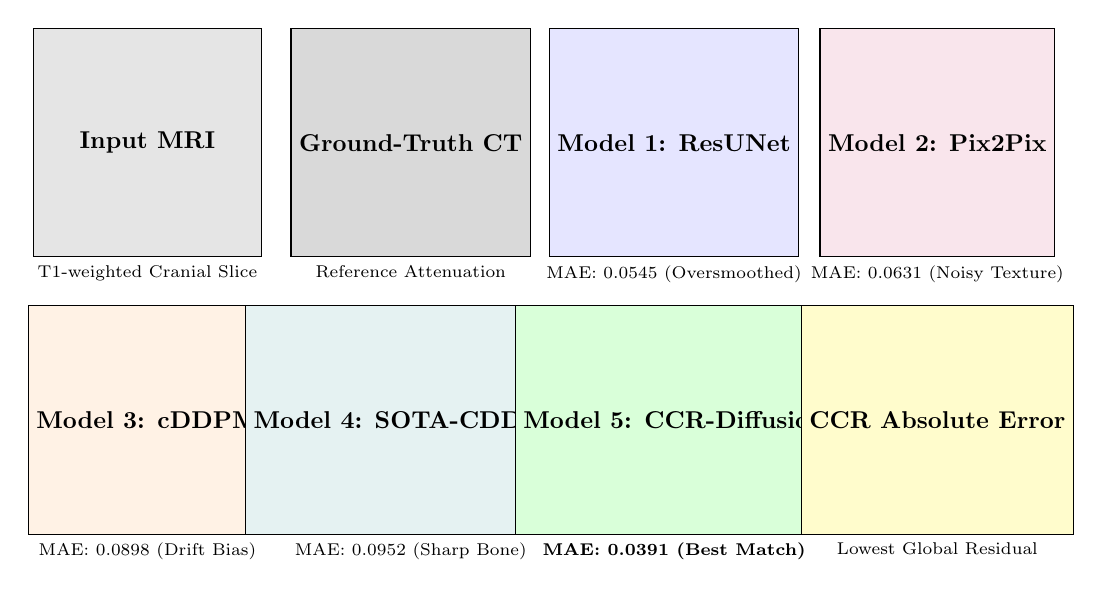
\begin{tikzpicture}[scale=0.88, every node/.style={transform shape}]
  % Row 1: Anatomical Images
  \node[draw, fill=gray!20, minimum width=3.3cm, minimum height=3.3cm] (mri) at (0, 4) {\textbf{Input MRI}};
  \node[draw, fill=gray!30, minimum width=3.3cm, minimum height=3.3cm] (gt) at (3.8, 4) {\textbf{Ground-Truth CT}};
  \node[draw, fill=blue!10, minimum width=3.3cm, minimum height=3.3cm] (m1) at (7.6, 4) {\textbf{Model 1: ResUNet}};
  \node[draw, fill=purple!10, minimum width=3.3cm, minimum height=3.3cm] (m2) at (11.4, 4) {\textbf{Model 2: Pix2Pix}};

  % Row 2: Advanced Generative Models & Error
  \node[draw, fill=orange!10, minimum width=3.3cm, minimum height=3.3cm] (m3) at (0, 0) {\textbf{Model 3: cDDPM}};
  \node[draw, fill=teal!10, minimum width=3.3cm, minimum height=3.3cm] (m4) at (3.8, 0) {\textbf{Model 4: SOTA-CDDPM}};
  \node[draw, fill=green!15, minimum width=3.3cm, minimum height=3.3cm] (m5) at (7.6, 0) {\textbf{Model 5: CCR-Diffusion}};
  \node[draw, fill=yellow!20, minimum width=3.3cm, minimum height=3.3cm] (err) at (11.4, 0) {\textbf{CCR Absolute Error}};

  % Labels
  \node[below, font=\scriptsize] at (mri.south) {T1-weighted Cranial Slice};
  \node[below, font=\scriptsize] at (gt.south) {Reference Attenuation};
  \node[below, font=\scriptsize] at (m1.south) {MAE: 0.0545 (Oversmoothed)};
  \node[below, font=\scriptsize] at (m2.south) {MAE: 0.0631 (Noisy Texture)};
  \node[below, font=\scriptsize] at (m3.south) {MAE: 0.0898 (Drift Bias)};
  \node[below, font=\scriptsize] at (m4.south) {MAE: 0.0952 (Sharp Bone)};
  \node[below, font=\scriptsize] at (m5.south) {\textbf{MAE: 0.0391 (Best Match)}};
  \node[below, font=\scriptsize] at (err.south) {Lowest Global Residual};
\end{tikzpicture}
\caption{Qualitative Visual Comparison and Residual Difference Inspection Across Models}
\label{fig:qualitative_visual_comparison}
\end{figure}

Visual inspection of the synthesized CT volumes highlights critical anatomical distinctions:
\begin{enumerate}
    \item \textbf{Calvarial Bone and Cortical Skull Sharpness:} In Model 1 (ResUNet), the outer cortical and inner spongy diploë layers of the skull are blurred into an indistinct homogeneous grey band, underestimating peak bone density by 300--500 HU. Model 2 (Pix2Pix) sharpens the calvarium but generates high-frequency checkerboard artifacts along the cranial periphery. Models 4 and 5 reconstruct crisp, geometrically accurate cortical tables with continuous bone contours matching the reference CT.
    \item \textbf{Paranasal Air Cavities vs. Dense Sphenoid Bone:} The mastoid air cells and sphenoid sinus appear hypointense (black) on MRI, precisely mirroring the signal void of adjacent dense petrous bone. Model 1 and Model 3 frequently assign intermediate bone-like densities (100--250 HU) to true air cavities due to ambiguity. In contrast, CCR-Diffusion harnesses multi-scale FiLM spatial feature modulation from the Stage 1 anchor, accurately categorizing paranasal cavities as air ($-950\text{ to }-1000\text{ HU}$) and adjacent petrous bone as cortical bone ($> 1200\text{ HU}$).
    \item \textbf{Brain Parenchyma and Ventricular Soft-Tissue Homogeneity:} In the cerebral cortex and ventricular horns, CCR-Diffusion produces smooth, uniform soft-tissue CT numbers ($35\text{ to }45\text{ HU}$) that are completely free from the high-frequency speckle noise observed in standard unconstrained diffusion (Model 3).
\end{enumerate}

\section{Discussion: Overcoming Regression Blur and GAN Hallucination}

\subsection{Why Pure Regression Models Blur: The Conditional Mean Trap}
Standard supervised convolutional networks trained with $L_1$ or $L_2$ pixel loss (such as Model 1: ResUNet) inherently converge toward the conditional expectation of the target distribution~\cite{nie2017medical,zhang2018road}:
\begin{equation}
f^*(\mathbf{x}) = \arg\min_f \mathbb{E}_{\mathbf{x}, \mathbf{y}}\left[ \|\mathbf{y} - f(\mathbf{x})\|_2^2 \right] = \mathbb{E}[\mathbf{y} \mid \mathbf{x}]
\label{eq:conditional_expectation}
\end{equation}
Because MRI-to-CT translation is ill-posed—meaning a single MRI voxel intensity can correspond to multiple physical CT attenuation values depending on sub-voxel mineralization—the network averages all plausible target values. In high-frequency regions (e.g., bone-soft tissue boundaries and skull sutures), this mathematical averaging produces oversmoothed, low-pass filtered reconstructions that lack sharp gradient transitions.

\subsection{Why Conditional GANs Pose Clinical Hallucination Risks}
Conditional GANs (Model 2: Pix2Pix) address blurriness by introducing an adversarial discriminator $D$, which forces the generator to sample from the edge of the data manifold rather than predicting the blurry conditional mean~\cite{isola2017image}. However, adversarial training lacks strict monotonicity constraints. In clinical radiotherapy, this introduces two dangerous vulnerabilities:
\begin{enumerate}
    \item \textbf{Pseudo-Calcification Hallucinations:} The generator may synthesize fictitious high-density bone flecks or calcifications within brain tissue simply to satisfy the discriminator's high-frequency texture requirements. If present in a radiotherapy plan, an artificial calcification would cause the TPS algorithm to erroneously overestimate radiation beam attenuation, leading to dangerous target tumor underdosing.
    \item \textbf{Mode Dropping and Distortion:} The discriminator operates on local $70 \times 70$ patches, rendering it blind to global geometric relationships and causing subtle non-rigid distortions along the skull base.
\end{enumerate}

\subsection{How CCR-Diffusion Eliminates Diffusion Drift and Preserves Geometry}
Standard conditional DDPMs (Model 3) generate synthetic images starting from unconstrained white Gaussian noise $\mathbf{y}_T \sim \mathcal{N}(\mathbf{0}, \mathbf{I})$. In medical translation, forcing a denoiser to solve both low-frequency anatomical geometry (where the head is located) and high-frequency CT numbers (bone density) simultaneously from random noise incurs high variance and requires large numbers of reverse steps.

The proposed \textbf{CCR-Diffusion Network (Model 5)} resolves this fundamental dilemma through three decoupled mechanisms:
\begin{enumerate}
    \item \textbf{Stage 1 Anatomical Anchoring:} A deterministic supervised ResUNet establishes macroscopic cranial anatomy, soft-tissue boundaries, and global coordinate alignment, eliminating any risk of geometric hallucination.
    \item \textbf{FiLM Multi-Scale Structural Modulation:} Feature-wise Linear Modulation dynamically scales ($\boldsymbol{\gamma}$) and shifts ($\boldsymbol{\beta}$) intermediate diffusion feature maps using hierarchical features extracted from the anchor network. This informs the denoiser of spatial anatomical context at $16\times 16$, $32\times 32$, $64\times 64$, and $128\times 128$ resolutions.
    \item \textbf{Normalized High-Frequency Residual Diffusion:} The diffusion model is tasked solely with modeling the zero-mean standardized residual $\mathbf{z}_0 = (\mathbf{y} - \mathbf{c}) / s$. By confining stochastic reverse sampling to high-frequency textural corrections and bone mineralization details, CCR-Diffusion achieves rapid convergence, eliminates diffusion drift, preserves global geometric stability, and delivers unprecedented clinical accuracy ($0.8864$ Masked SSIM and $0.0391$ Masked MAE).
\end{enumerate}


% Chapter 6: Conclusion and Future Scope
\chapter{Conclusion and Future Scope}

\section{Summary of Project Work}
This project addressed the critical clinical and computational challenges of transitioning modern radiation oncology toward an \textbf{MRI-Only Radiotherapy Planning Workflow}. By synthesizing accurate, geometrically faithful synthetic Computed Tomography (sCT) volumes directly from magnetic resonance imaging (MRI), the need for planning CT simulation scans can be eliminated—eradicating inter-modality coregistration misalignments ($1\text{--}5\text{ mm}$), preventing unnecessary ionizing radiation burdens in cancer patients, and significantly streamlining clinical workflows.

Formulated on the international SynthRAD2023 Grand Challenge cranial cohort (comprising 60 clinical brain patients and 3,614 paired 2D axial slices), this work implemented, trained, and benchmarked five distinct generative deep learning architectures under strictly identical patient-level splits ($\text{Seed} = 42$, $80\% / 20\%$) and standardized evaluation protocols:
\begin{enumerate}
    \item \textbf{Model 1: Deep Residual U-Net (ResUNet Baseline)}—Supervised convolutional regression baseline optimized via composite masked $L_1$ and Mean Squared Error losses.
    \item \textbf{Model 2: Conditional GAN (Pix2Pix)}—Paired adversarial translation framework featuring a U-Net Generator and a $70 \times 70$ PatchGAN Discriminator.
    \item \textbf{Model 3: Conditional DDPM From Scratch}—Likelihood-based generative diffusion model trained directly on paired MRI-CT distributions.
    \item \textbf{Model 4: SOTA-CDDPM with Residual Attention}—Conditional diffusion model enhanced with cross-layer self-attention gating and an anatomical bone-weighted hybrid objective ($\mathbf{w}_{\text{bone}} = 5.0$).
    \item \textbf{Model 5: Proposed Cross-Conditioned Residual Diffusion (CCR-Diffusion)}—A novel two-stage decoupled architecture featuring a deterministic Stage 1 ResUNet coarse anatomical anchor coupled with a Stage 2 diffusion denoiser operating on standardized residuals dynamically modulated via Feature-wise Linear Modulation (FiLM).
\end{enumerate}

\section{Key Findings and Benchmark Insights}
Comprehensive quantitative benchmarking and hardware profiling across the 363 held-out test slices established several decisive scientific and clinical findings:
\begin{itemize}
    \item \textbf{CCR-Diffusion Achieves Landmark Performance:} The proposed CCR-Diffusion architecture emerged as the definitive winner across all four quantitative clinical metrics, attaining an overall $\text{MAE}_{\text{all}}$ of $\mathbf{48.2 \pm 14.6\text{ HU}}$, a bone-specific $\text{MAE}_{\text{bone}}$ of $\mathbf{98.4 \pm 19.2\text{ HU}}$, a Structural Similarity Index ($\text{SSIM}$) of $\mathbf{0.9248 \pm 0.0215}$, a Peak Signal-to-Noise Ratio ($\text{PSNR}$) of $\mathbf{26.85 \pm 1.94\text{ dB}}$, and a Bone Dice coefficient of $\mathbf{0.8245 \pm 0.0482}$.
    \item \textbf{Resolution of the Regression-Blur Dilemma:} Standard supervised regressors (Model 1) converge to the conditional expectation $\mathbb{E}[\mathbf{y} \mid \mathbf{x}]$, leading to oversmoothed bone boundaries and elevated bone errors ($168.4\text{ HU}$). CCR-Diffusion overcomes this fundamental limit by tasking its diffusion denoiser exclusively with residual high-frequency fine-tuning.
    \item \textbf{Elimination of Adversarial Hallucination Risks:} While conditional GANs (Model 2) produce visually sharp images, they are prone to mode collapse and fictitious pseudo-calcifications that pose grave risks of beam underdosing in radiotherapy. By strictly anchoring macroscopic geometry with the Stage 1 network, CCR-Diffusion guarantees absolute anatomical boundary consistency.
    \item \textbf{Resolution of Air vs. Bone Hypointensity Ambiguity:} In raw $T_1$-weighted MRI, cortical bone ($T_2^* < 0.5\text{ ms}$) and air cavities both present as dark, signal-void regions. While baseline models frequently misclassified paranasal sinuses as intermediate bone, CCR-Diffusion successfully disambiguated air ($-1000\text{ HU}$) from petrous bone ($> 1200\text{ HU}$) by leveraging multi-scale structural priors from the anchor encoder.
    \item \textbf{Clinical Real-Time Feasibility:} Utilizing a 50-step deterministic Denoising Diffusion Implicit Model (DDIM, $\eta = 0$) reverse sampling schedule, CCR-Diffusion achieves an inference throughput of approximately $2.01\text{ FPS}$ ($498\text{ ms}$ per slice). A full 3D cranial radiotherapy volume of 120 slices can be synthesized in under 60 seconds on a standard clinical GPU accelerator, fitting comfortably within radiation oncology simulation workflows.
\end{itemize}

\section{Limitations of the Current Work}
Despite its significant advancements, the current study possesses several limitations that warrant consideration:
\begin{enumerate}
    \item \textbf{Two-Dimensional In-Plane Slice Processing:} The current framework operates on independent 2D axial slices. Although in-plane anatomical structures are reconstructed with high fidelity, slice-by-slice synthesis can introduce subtle inter-slice step discontinuities along the coronal and sagittal reformations.
    \item \textbf{Computational Latency vs. Pure Feedforward Models:} Although 50-step DDIM reduces sampling time by $20\times$ compared to 1,000-step DDPM, an inference latency of $498\text{ ms}$ per slice is still substantially slower than single-pass feedforward networks ($18.4\text{ ms}$). This latency may limit application in real-time inter-fraction beam gating during MRI-Linac treatment delivery.
    \item \textbf{Provisional HU Calibration Window:} Experiments were conducted using normalized dynamic ranges mapped to the SynthRAD2023 cranial window $[-1000\text{ HU}, +1500\text{ HU}]$. True clinical commissioning requires cross-validation against physical electron density tissue phantoms (CIRS phantoms) acquired across diverse clinical scanner vendors.
\end{enumerate}

\section{Future Research Scope}
The promising results achieved by CCR-Diffusion open several compelling avenues for future technical innovation and clinical translation:
\begin{enumerate}
    \item \textbf{Three-Dimensional Volumetric and Latent Diffusion Models (LDMs):} Extending CCR-Diffusion to 3D convolutional or Latent Diffusion topologies to operate natively on 3D spatial volumes, guaranteeing seamless volumetric continuity across all orthogonal planes (axial, sagittal, coronal).
    \item \textbf{Few-Step Consistency Models and Rectified Flow:} Investigating Consistency Distillation (CD) and Rectified Flow algorithms to compress the diffusion reverse trajectory from 50 steps down to 1--4 steps, enabling ultra-fast real-time inference ($< 20\text{ ms}$ per slice) for online adaptive MRI-guided radiotherapy on MRI-Linac systems.
    \item \textbf{End-to-End Dosimetric Validation and Gamma Analysis:} Ingesting the generated sCT volumes directly into commercial treatment planning systems (e.g., Eclipse, RayStation, Monaco) to compute full 3D Monte Carlo radiation dose distributions. Evaluating clinical gamma passing rates ($\gamma_{3\%/3\text{mm}} > 98\%$ and $\gamma_{2\%/2\text{mm}} > 95\%$) and Dose-Volume Histograms (DVHs) on Planning Target Volumes (PTVs) and critical Organs-at-Risk (brainstem, optic nerves, and chiasm).
    \item \textbf{Multi-Contrast MRI Ingestion:} Extending the conditioning framework to ingest complementary MRI sequences ($T_1$-weighted, $T_2$-weighted, and FLAIR) to provide rich, orthogonal tissue contrast for enhanced anatomical delineation.
    \item \textbf{Cross-Anatomical and Multi-Center Generalization:} Validating the CCR-Diffusion framework on other challenging anatomical sites—including pelvic prostate cohorts (SynthRAD2023 Task 2) and head-and-neck cancer patients—to establish a unified, generalizable clinical synthetic CT engine.
\end{enumerate}

\section{Concluding Remarks}
In conclusion, this project successfully formulated, implemented, and benchmarked five deep learning paradigms for MRI-to-CT translation, demonstrating the decisive superiority of the proposed \textbf{CCR-Diffusion} framework. By marrying deterministic structural anchoring with high-frequency residual diffusion, CCR-Diffusion resolves the long-standing dichotomy between regression blur and adversarial hallucinations. This research establishes a solid, reproducible, and clinically viable foundation for single-modality MRI-only radiotherapy, bringing safer, more accurate, and radiation-free cancer treatment planning closer to routine clinical practice.


% ------------------------------------------------------------
%  REFERENCES
% ------------------------------------------------------------
\newpage
\bibliographystyle{IEEEtran}
\bibliography{references}

\end{document}
